\newpage
\section{Auswertung}
\label{sec:Auswertung}
 
Die Versuche wurden aus Zeitgründen nur mit dem Computer und nicht mit dem Oszilloskop durchgeführt. Analysiert wurden die Ergebnisse mittels der Python Module matplotlib \cite{matplotlib}, numpy \cite{numpy}, scipy \cite{scipy} und uncertainties \cite{uncertainties}.

\subsection{1D-Festkörper}

Das Frequenzspektrum, in dem gemessen wird, geht von \SI{0.1}{\kilo\hertz} bis \SI{12}{\kilo\hertz}. 
Die Peaks der Resonanzen sind für die Messungen für ein bis zwölf Zylinder in Tabelle \ref{tab:rohr} aufgetragen. Aus der Steigung der Ausgleichsgeraden durch den Nullpunkt lässt sich mit Gleichung \ref{eq:speed} die Schallgeschwindigkeit bestimmen. Der Steigungsparameter ergibt sich zu \SI{342.6(7)}{\meter\per\second}. 
Der Literaturwert der Schallgeschwindigkeit beträgt nach \cite{speed} \SI{343.38}{\metre\per\second} bei einer angenommenen Raumtemperatur von \SI{20}{\celsius}. 

\begin{table}\caption{Die Anzahl der Zylinder $n$, die Gesamtlänge des zusammengesetzten Systems $L$, die jeweiligen Resonanzfrequenzen $f_{1,2}$ und die Differenz $\Delta f$ sind hier aufgetragen.}
    \label{tab:rohr}
    \centering
    \sisetup{round-mode = places, round-integer-to-decimal=true}
     \begin{tabular}{c c | c c | c} 
        %\begin{tabular}{c | c c c  | c c c}  
    \toprule
{$n$} & {$L / \si{\milli\metre}$} & {$f_1 / \si{\kilo\hertz}$} & {$f_2 / \si{\kilo\hertz}$} & {$\Delta f / \si{\kilo\hertz}$} \\
\midrule
1     &    50   &  6885  &  10295 &   3410  \\
2     &   100   &  6900  &  8620  &   1720  \\
3     &   150   &  6910  &  8065  &   1155  \\ 
4     &   200   &  6910  &  7775  &   865  \\
5     &   250   &  6915  &  7605  &   690  \\
6     &   300   &  6915  &  7490  &   575  \\  
7     &   350   &  6915  &  7410  &   495  \\  
8     &   400   &  6915  &  7350  &   435  \\  
9     &   450   &  6915  &  7300  &   385  \\  
10    &   500   &  6915  &  7265  &   350  \\    
11    &   550   &  6915  &  7235  &   320  \\  
12    &   600   &  6915  &  7210  &   295  \\

\bottomrule
\end{tabular}\end{table}

\begin{figure}
    \centering
    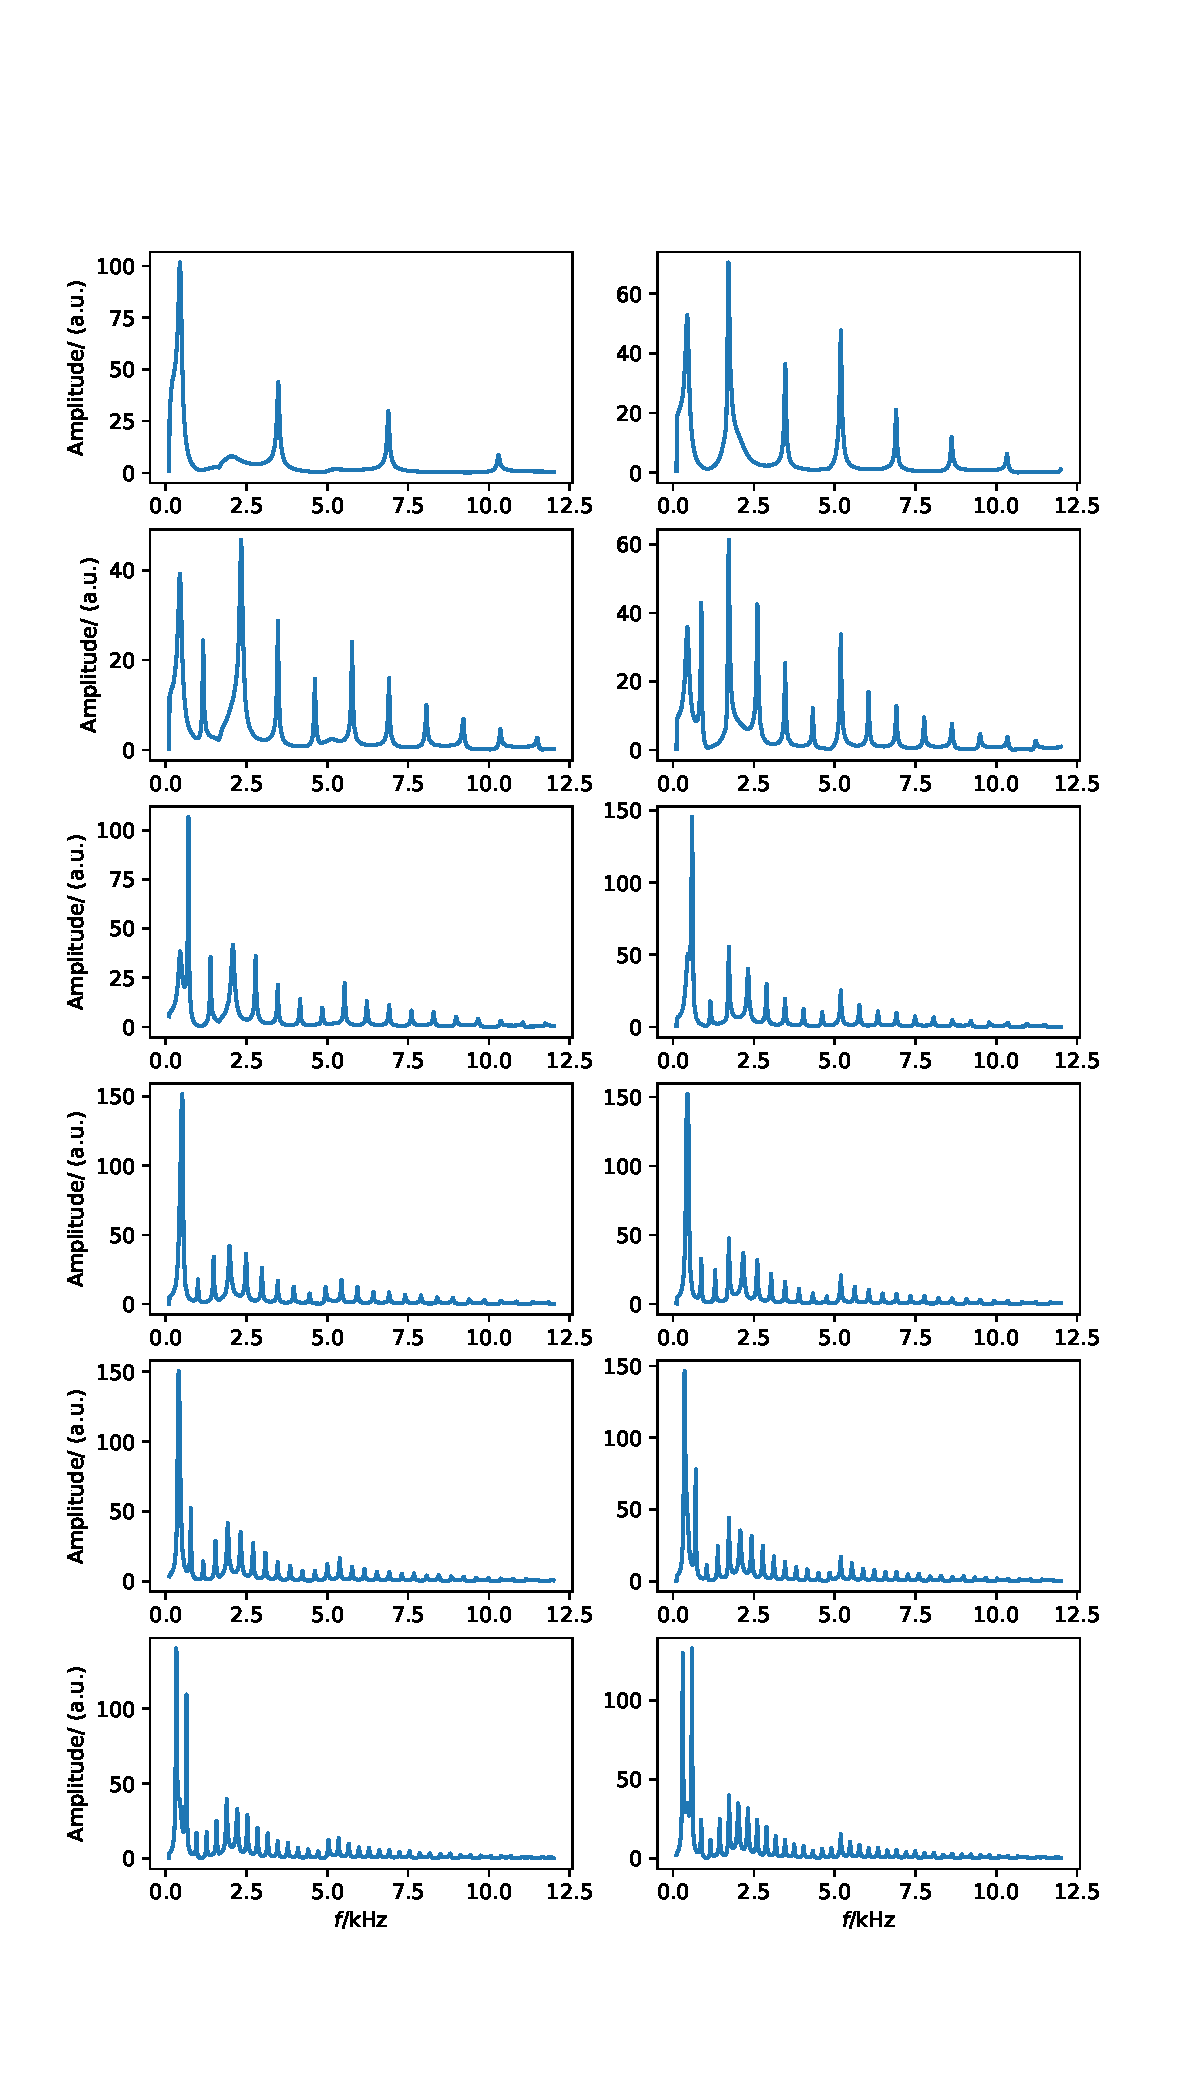
\includegraphics[width=0.8\textwidth]{plots/A_2.pdf}
    \caption{Die doppelte inverse Länge des Rohrresonators ist hier gegen die Differenz zwischen den resonanten Frequenzen $\Delta f$ aufgetragen.}
    \label{fig:speed}
\end{figure}

Das Spektrum für einen einzelnen Zylinder der Länge $\SI{75}{\milli\metre}$ ist in Abb. \ref{fig:A3} zu sehen.
\begin{figure}
    \centering
    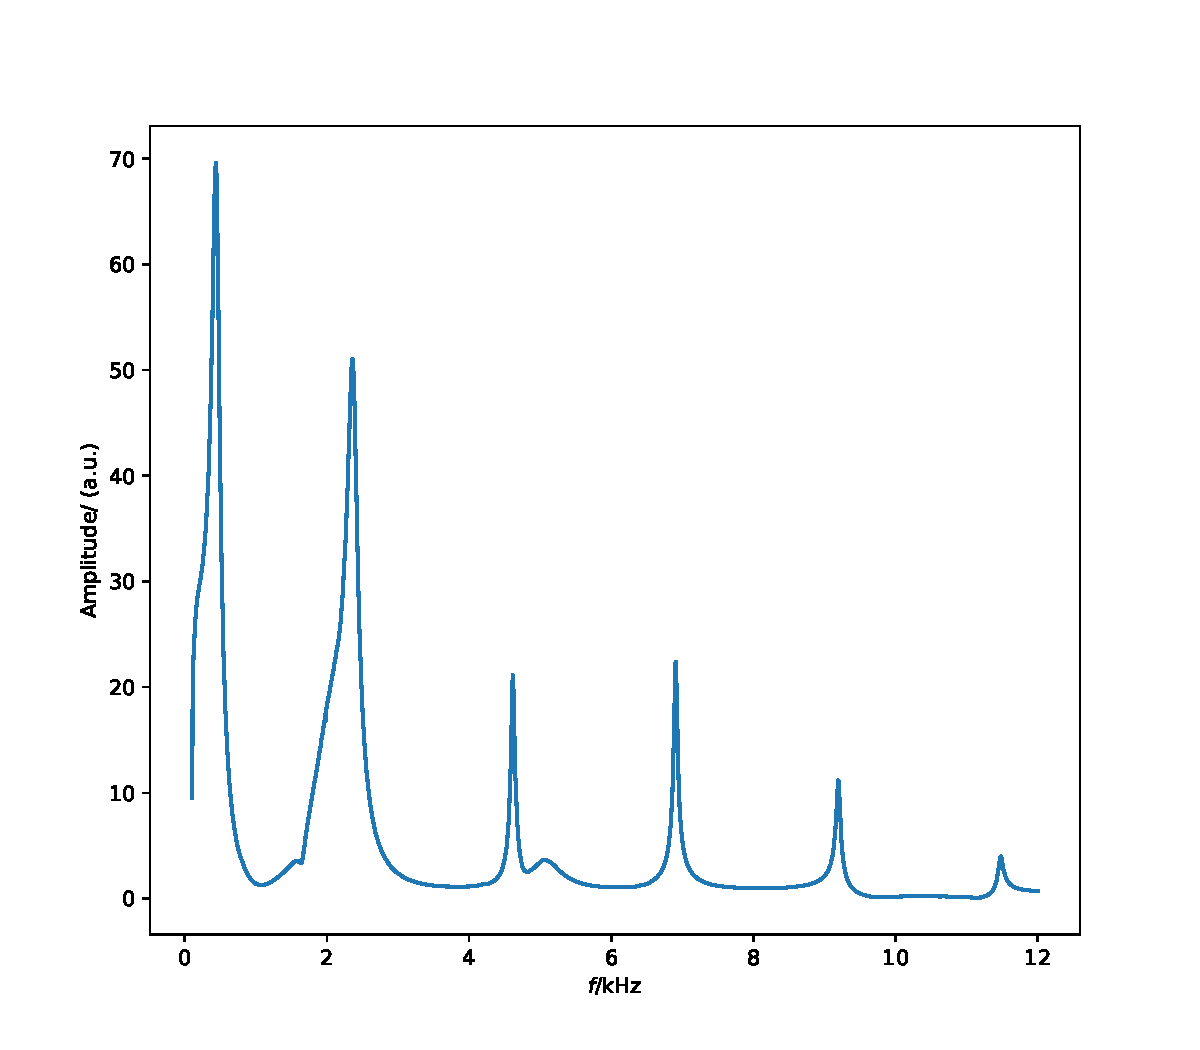
\includegraphics[width=0.8\textwidth]{plots/A_3.pdf}
    \caption{Das Frequenzspektrum für einen Zylinder mit einer Länge von \SI{7.5}{\centi\metre}.}
    \label{fig:A3}
\end{figure}

Der Abstand zwischen den Peaks beträgt hier \SI{2285}{\hertz}. 
Mit der zuvor bestimmten Schallgeschwindigkeit von \SI{342.6(7)}{\meter\per\second} ergibt sich für die Frequenzdifferenz ein Wert von \SI{2284(5)}{\hertz}.

Das Spektrum für \num{2}, \num{4} und \num{10} Zylinder mit einer \SI{16}{\milli\meter} Blende zwischen den einzelnen Segmenten ist in Abb. \ref{fig:spec10} zu sehen. Damit lässt sich das Verhalten für ein gekoppeltes System beschreiben. Wie erwartet bilden sich bei mehr Segmenten Bänder mit einer Anzahl an Peaks entsprechend der Anzahl der Segmente, die kontinuierlich werden für eine unendliche Anzahl an Segmenten. 

\begin{figure}
    \centering
    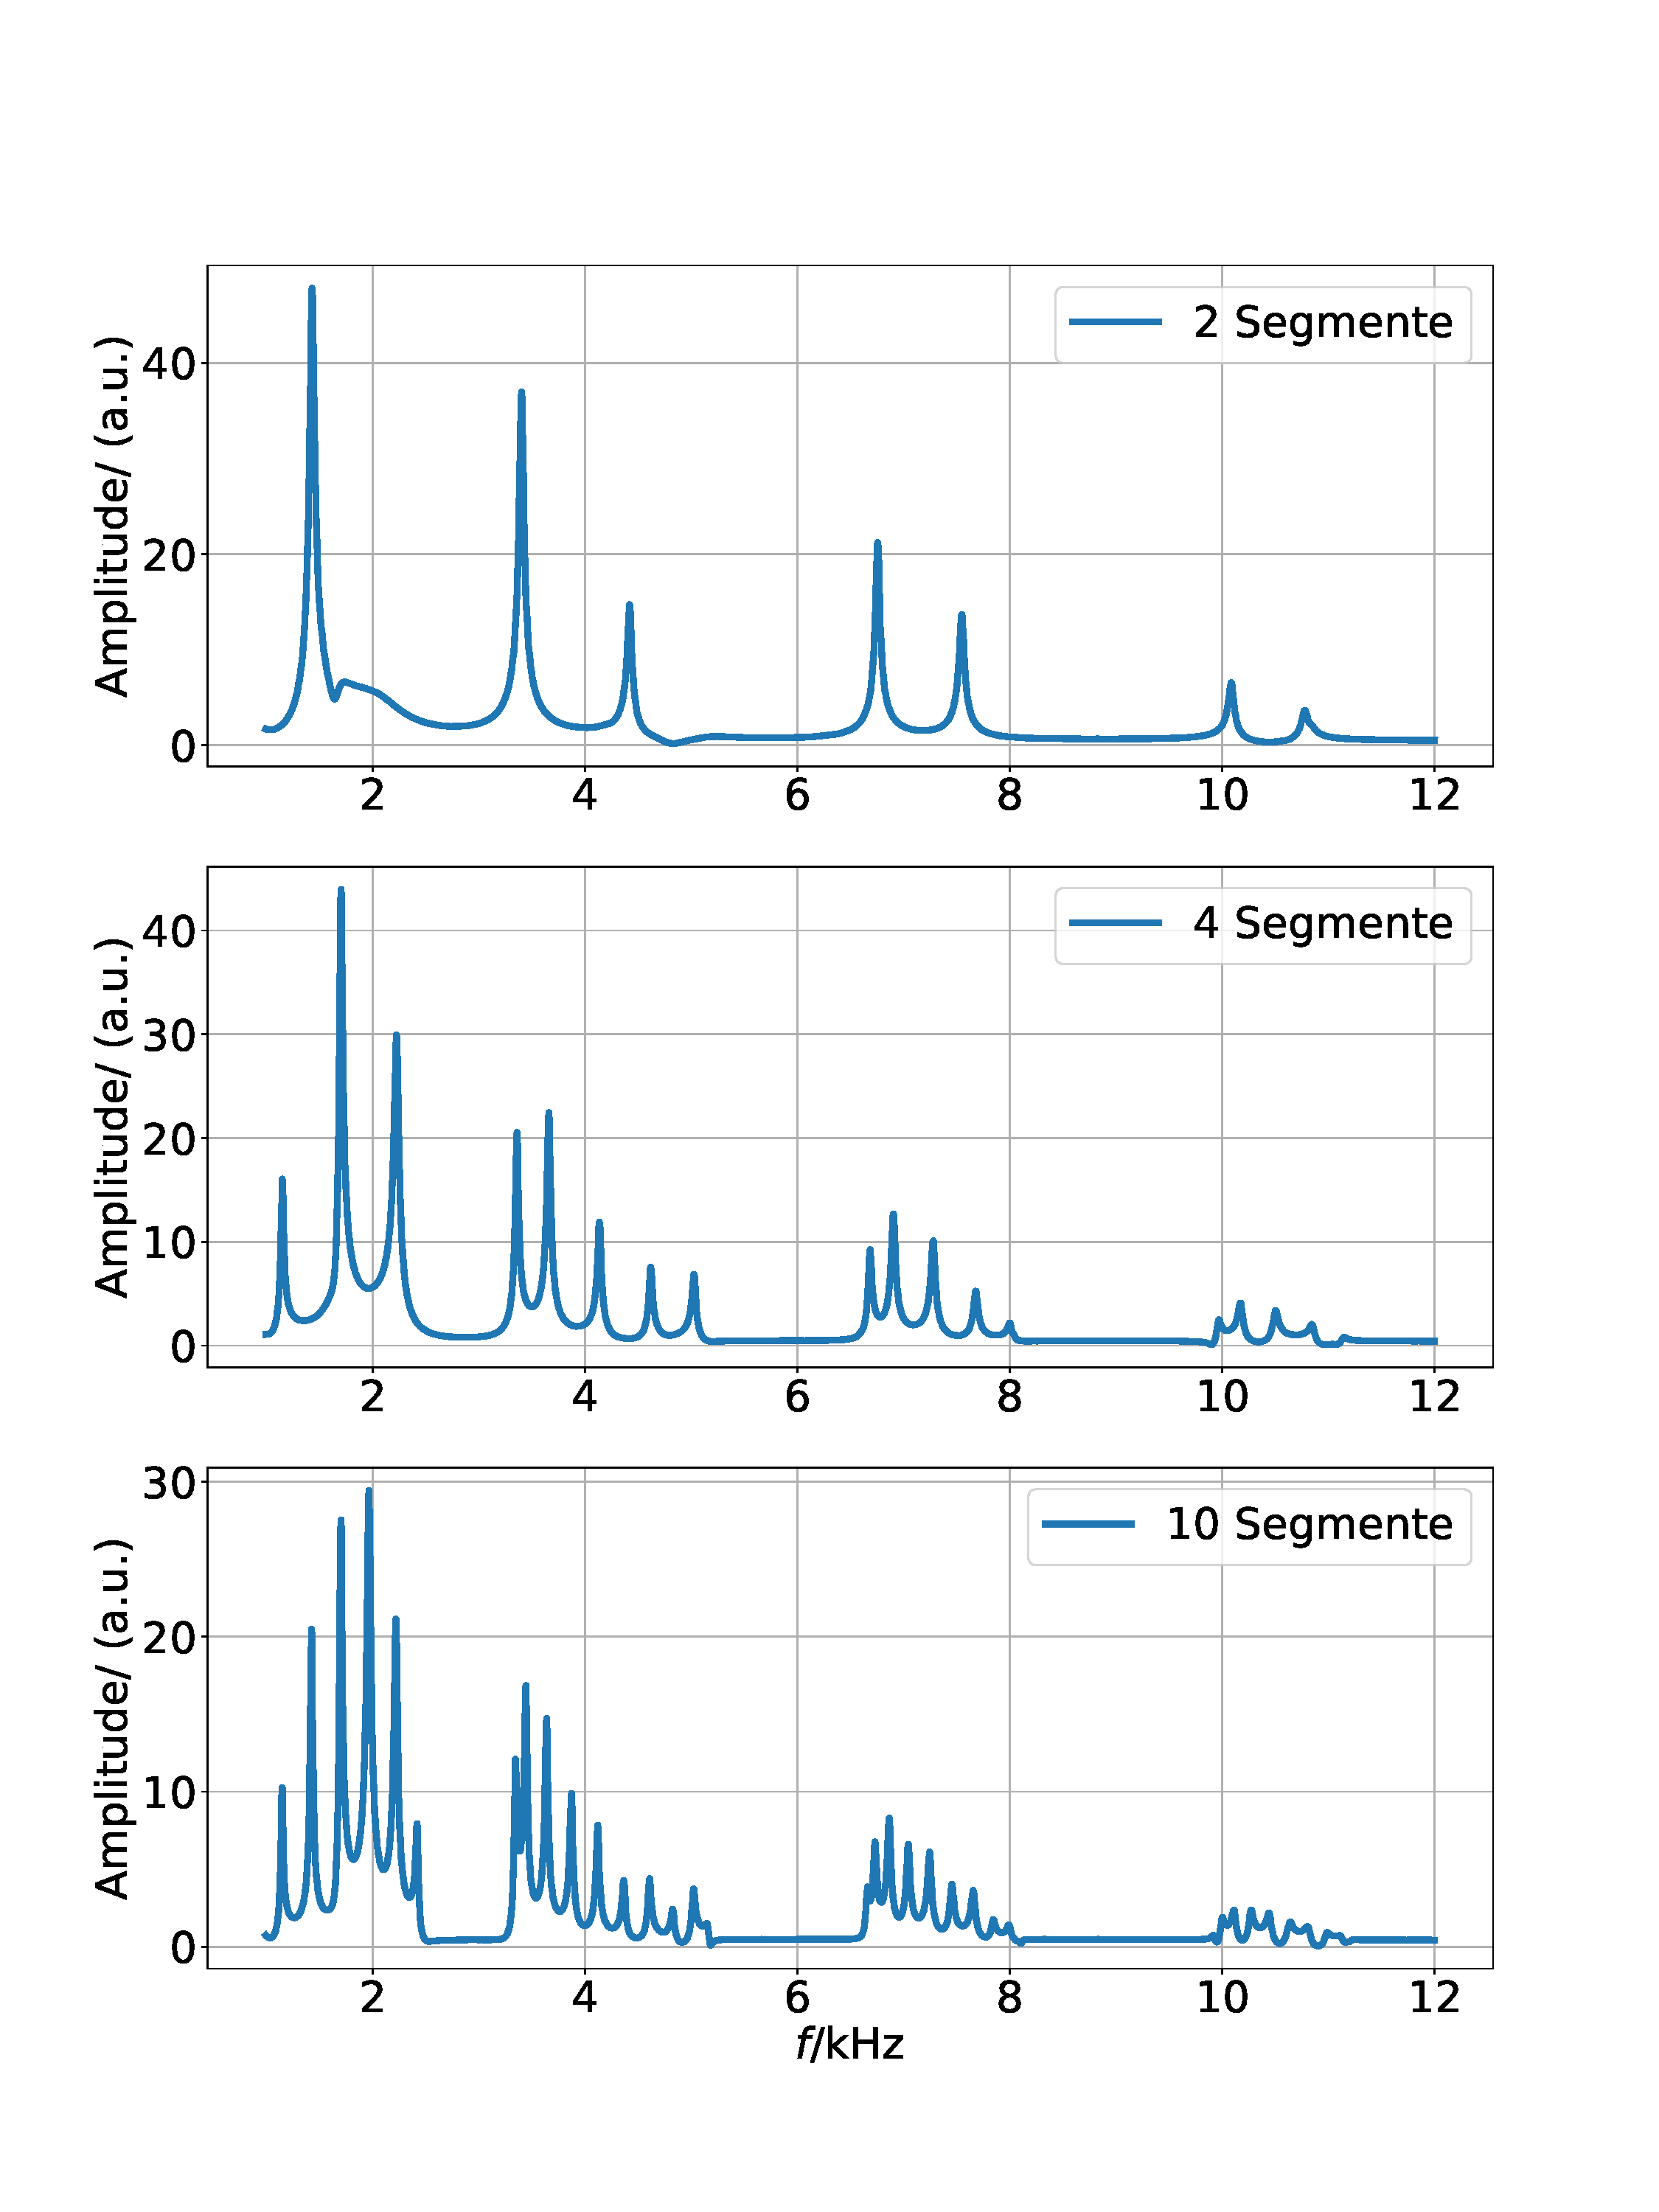
\includegraphics[width=0.65\textwidth]{plots/B_1.pdf}
    \caption{Das Frequenzspektrum für \num{2}, \num{4} und \num{10} Zylinder mit jeweils einer Länge von \SI{50}{\milli\metre}. Zwischen den Zylindern befinden sich jeweils Blenden mit einem Durchmesser von \SI{16}{\milli\metre}.}
    \label{fig:spec10}
\end{figure}

Das Ganze wird erneut für \num{2}, \num{4} und \num{10} Zylinder mit Blenden des Durchmessers \SI{10}{\milli\meter} und \SI{13}{\milli\meter} durchgeführt. In der Analogie entspricht das einer schwächeren Kopplung zwischen den einzelnen Segmenten. Die Spektren sind in Abb. \ref{fig:spec10_13} zu sehen. 

\begin{figure}
    \centering
    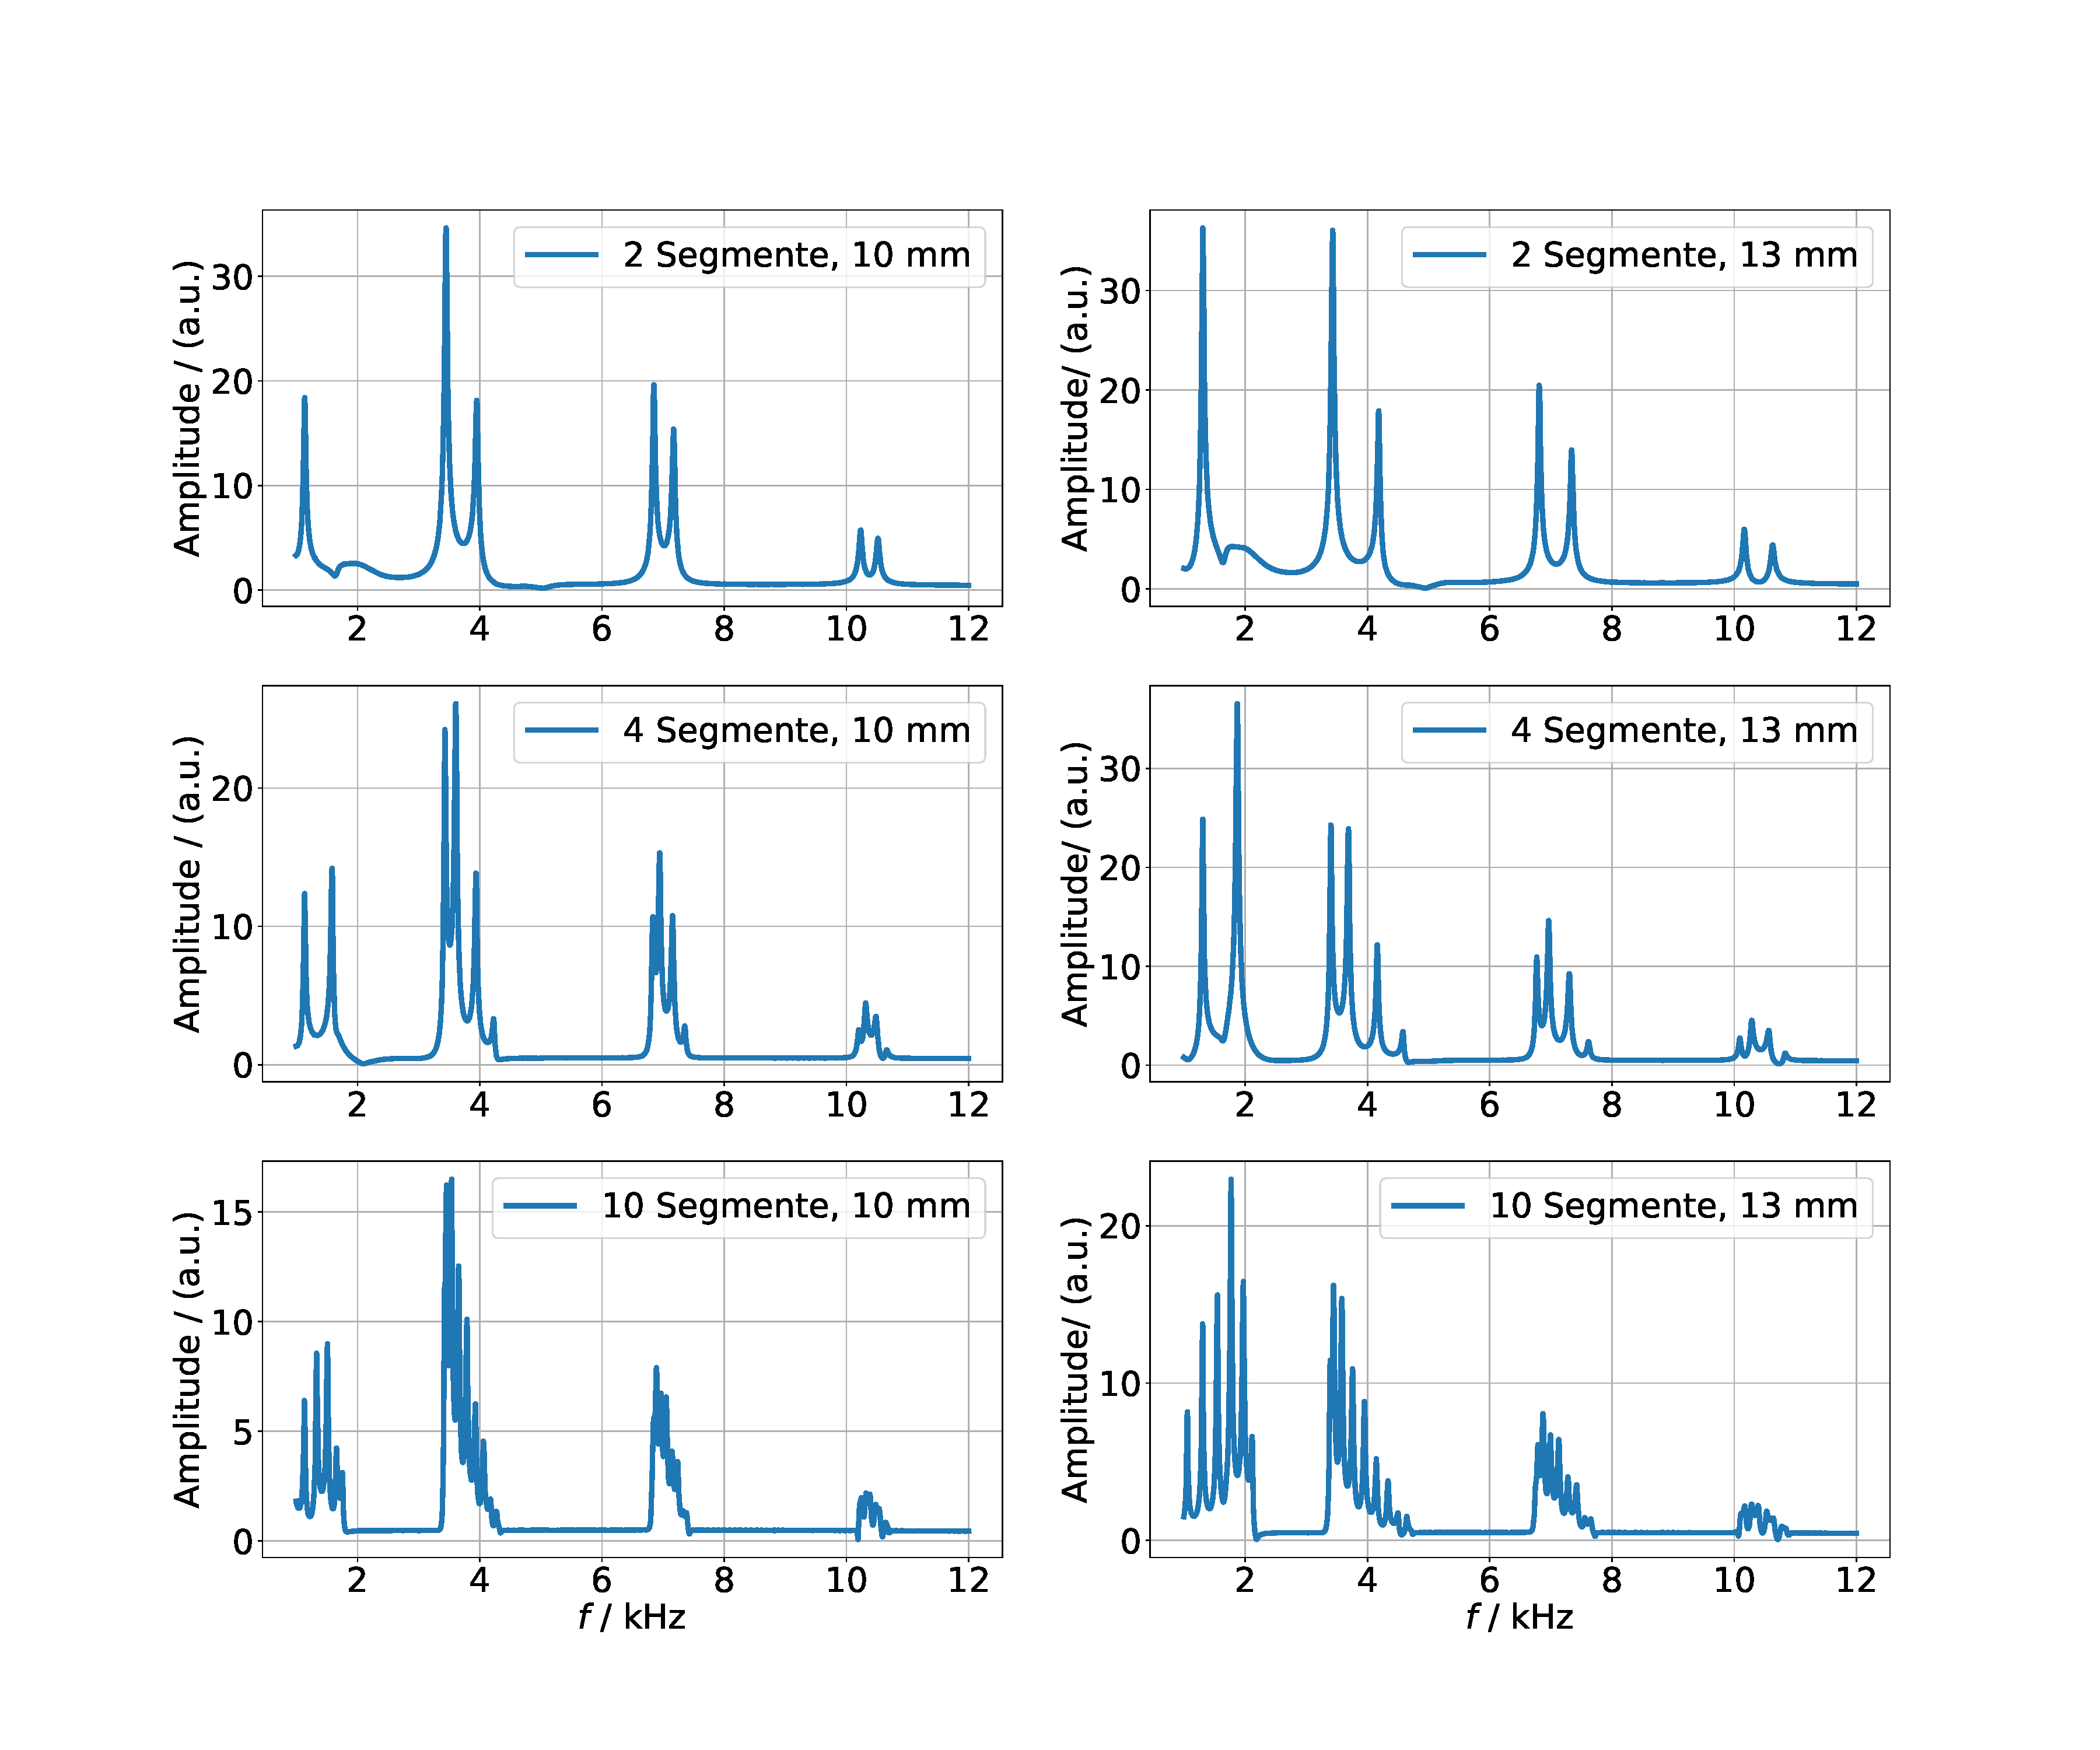
\includegraphics[width=\textwidth]{plots/B_3.pdf}
    \caption{Das Frequenzspektrum für 2, 4 und 10 Zylinder mit jeweils einer Länge von \SI{50}{\milli\metre} mit Blendendurchmesser von \SI{10}{\milli\metre} und \SI{13}{\milli\metre}.}
    \label{fig:spec10_13}
\end{figure}

Die Messung wurde erneut variiert, indem einer der \num{10} Zylinder mit einer Länge von \SI{50}{\milli\meter} durch einen Zylinder anderer Länge ersetzt wurde. Die neuen Längen sind \SI{75}{\milli\meter}, \SI{62.5}{\milli\meter} und \SI{37.5}{\milli\meter}. In der Analogie entspricht dies einem Defekt in dem System.
%Verbesserung:
Es entstehen zusätzliche Zustände zwischen den Bändern analog zur Dotierung von Halbleitern.
Bei dem Pendel entspräche dieser Fall einem Element in der Kette, das eine größere bzw. kleinere Masse hat. 
Die Veränderung ist in der linken Spalte von Abb. \ref{fig:var4} zu sehen.

Eine Kette aus 10 Zylindern wurde abwechselnd aus \SI{50}{\milli\meter} und \SI{75}{\milli\meter} Zylindern mit \SI{16}{\milli\meter} Blenden zusammengesetzt.
Das Ergebnis ist als Vergleich zu einem einzelnen Zylinder der Länge \SI{50}{\milli\metre} und \SI{75}{\milli\metre} in der rechten Spalte von Abb. \ref{fig:var4} zu sehen. In der Analogie der Pendel entspricht dieser Fall einem Pendel mit alternierenden Massen der Segmente.
%Verbesserung:
Man kann die Bänder den einzelnen Resonanzen zuordnen, weil die Resonatoren sich in bestimmten Schwingungen genau so verhalten, als wären die Segmente der jeweils anderen Größe dazwischen gar nicht da. Deshalb befinden sich die Bänder dann an der gleichen Stelle. Wenn mehr der anderen Segmente mitschwingen, entsteht das ganze Band.
 
\begin{figure}
    \centering
    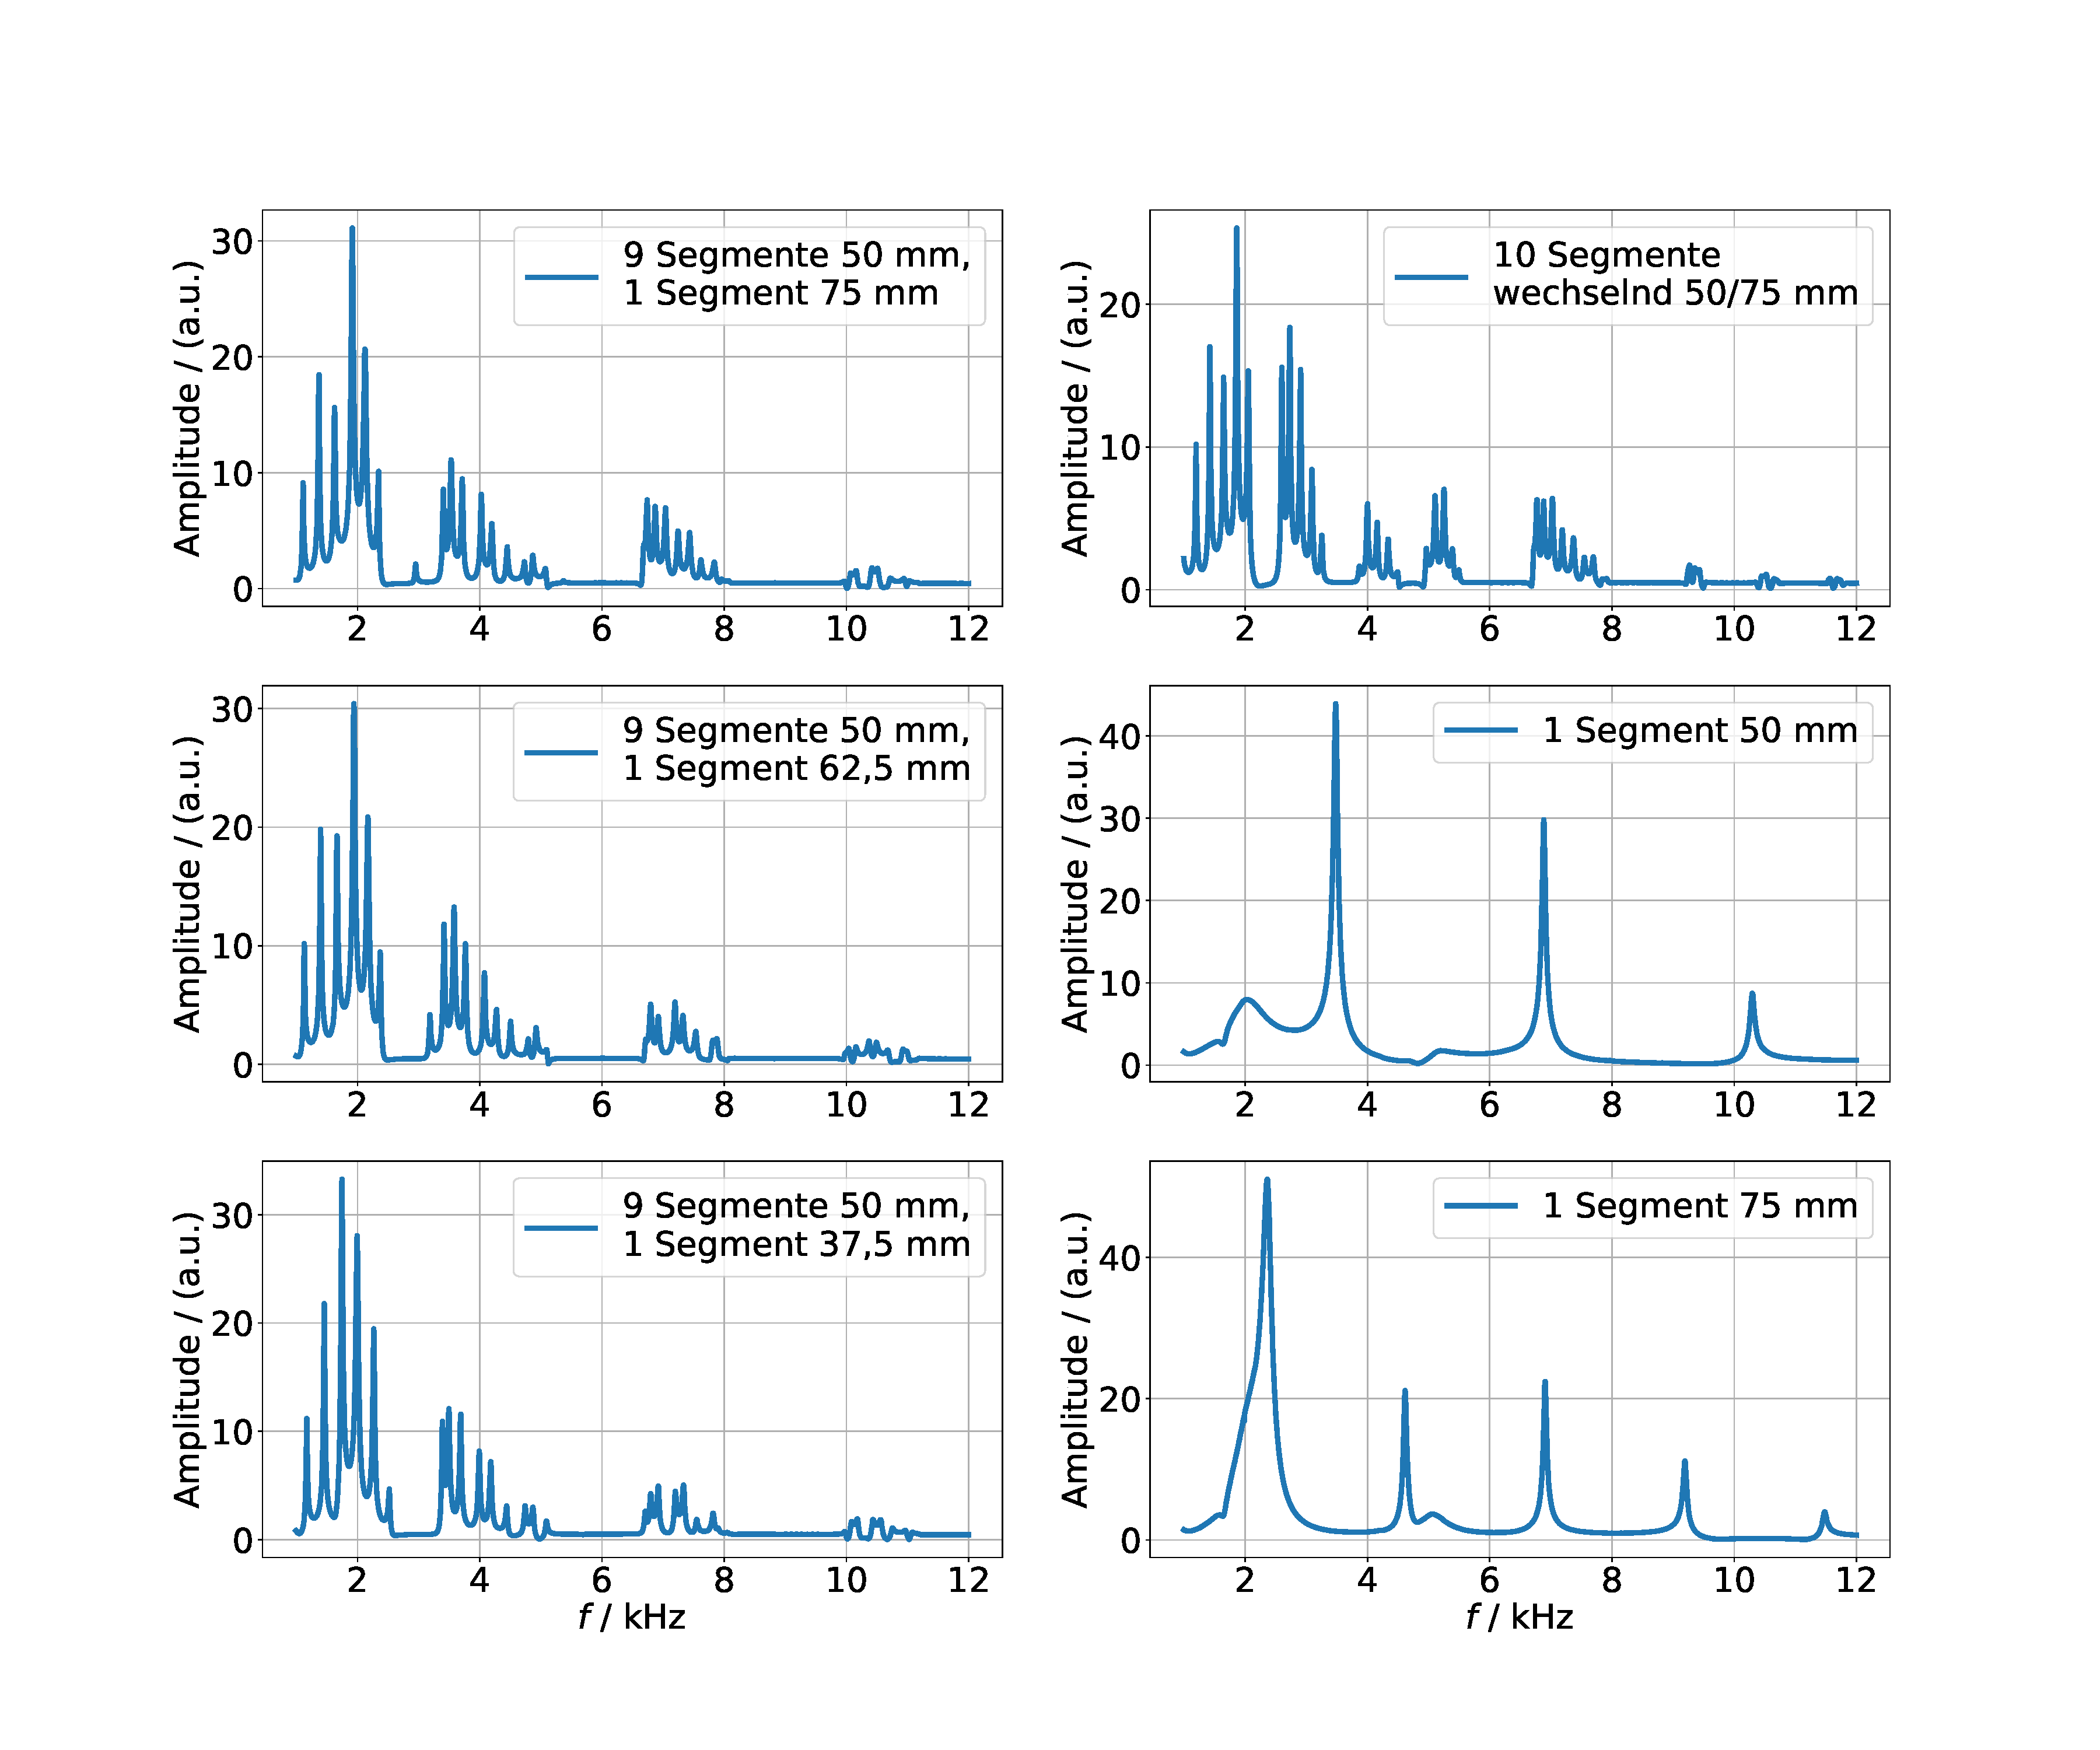
\includegraphics[width=\textwidth]{plots/B_5.pdf}
    \caption{Das Frequenzspektrum für 9 Zylinder mit jeweils einer Länge von \SI{50}{\milli\metre} und einem Zylinder der Länge \SI{75}{\milli\metre}, \SI{62.5}{\milli\metre}, \SI{37.5}{\milli\metre} ist in der linken Spalte aufgetragen. Dazwischen befinden sich Blenden. Der Blendendurchmesser beträgt \SI{16}{\milli\metre}. Zwischen den Bändern sind zusätzliche Zustände analog zur Dotierung von Halbleitern zu sehen. %<- Verbesserung
    Das Frequenzspektrum einer Kette aus 10 Zylindern, deren Längen abwechselnd \SI{50}{\milli\metre} und \SI{75}{\milli\metre} betragen, ist in der rechten Spalte zu sehen. Der Blendendurchmesser der zwischen den Zylindern platzierten Blenden beträgt \SI{16}{\milli\metre}. Darunter ist vergleichsweise das Frequenzspektrum für einen einzelnen Zylinder der Länge \SI{50}{\milli\metre} und für einen Zylinder der Länge \SI{75}{\milli\metre} aufgetragen.}
    \label{fig:var4}
\end{figure}

Als letzte Variation wurden \num{8} Zylinder der Länge \SI{50}{\milli\metre} verwendet, zwischen die abwechselnd Blenden mit Durchmesser \SI{13}{\milli\metre} und \SI{16}{\milli\metre} gesetzt wurden. 
Das Ergebnis ist in Abb. \ref{fig:var5} zu sehen. In der Analogie der Pendel entspricht dieser Fall einem Pendel mit alternierenden Kopplungskonstanten zwischen den Segmenten.

\begin{figure}
    \centering
    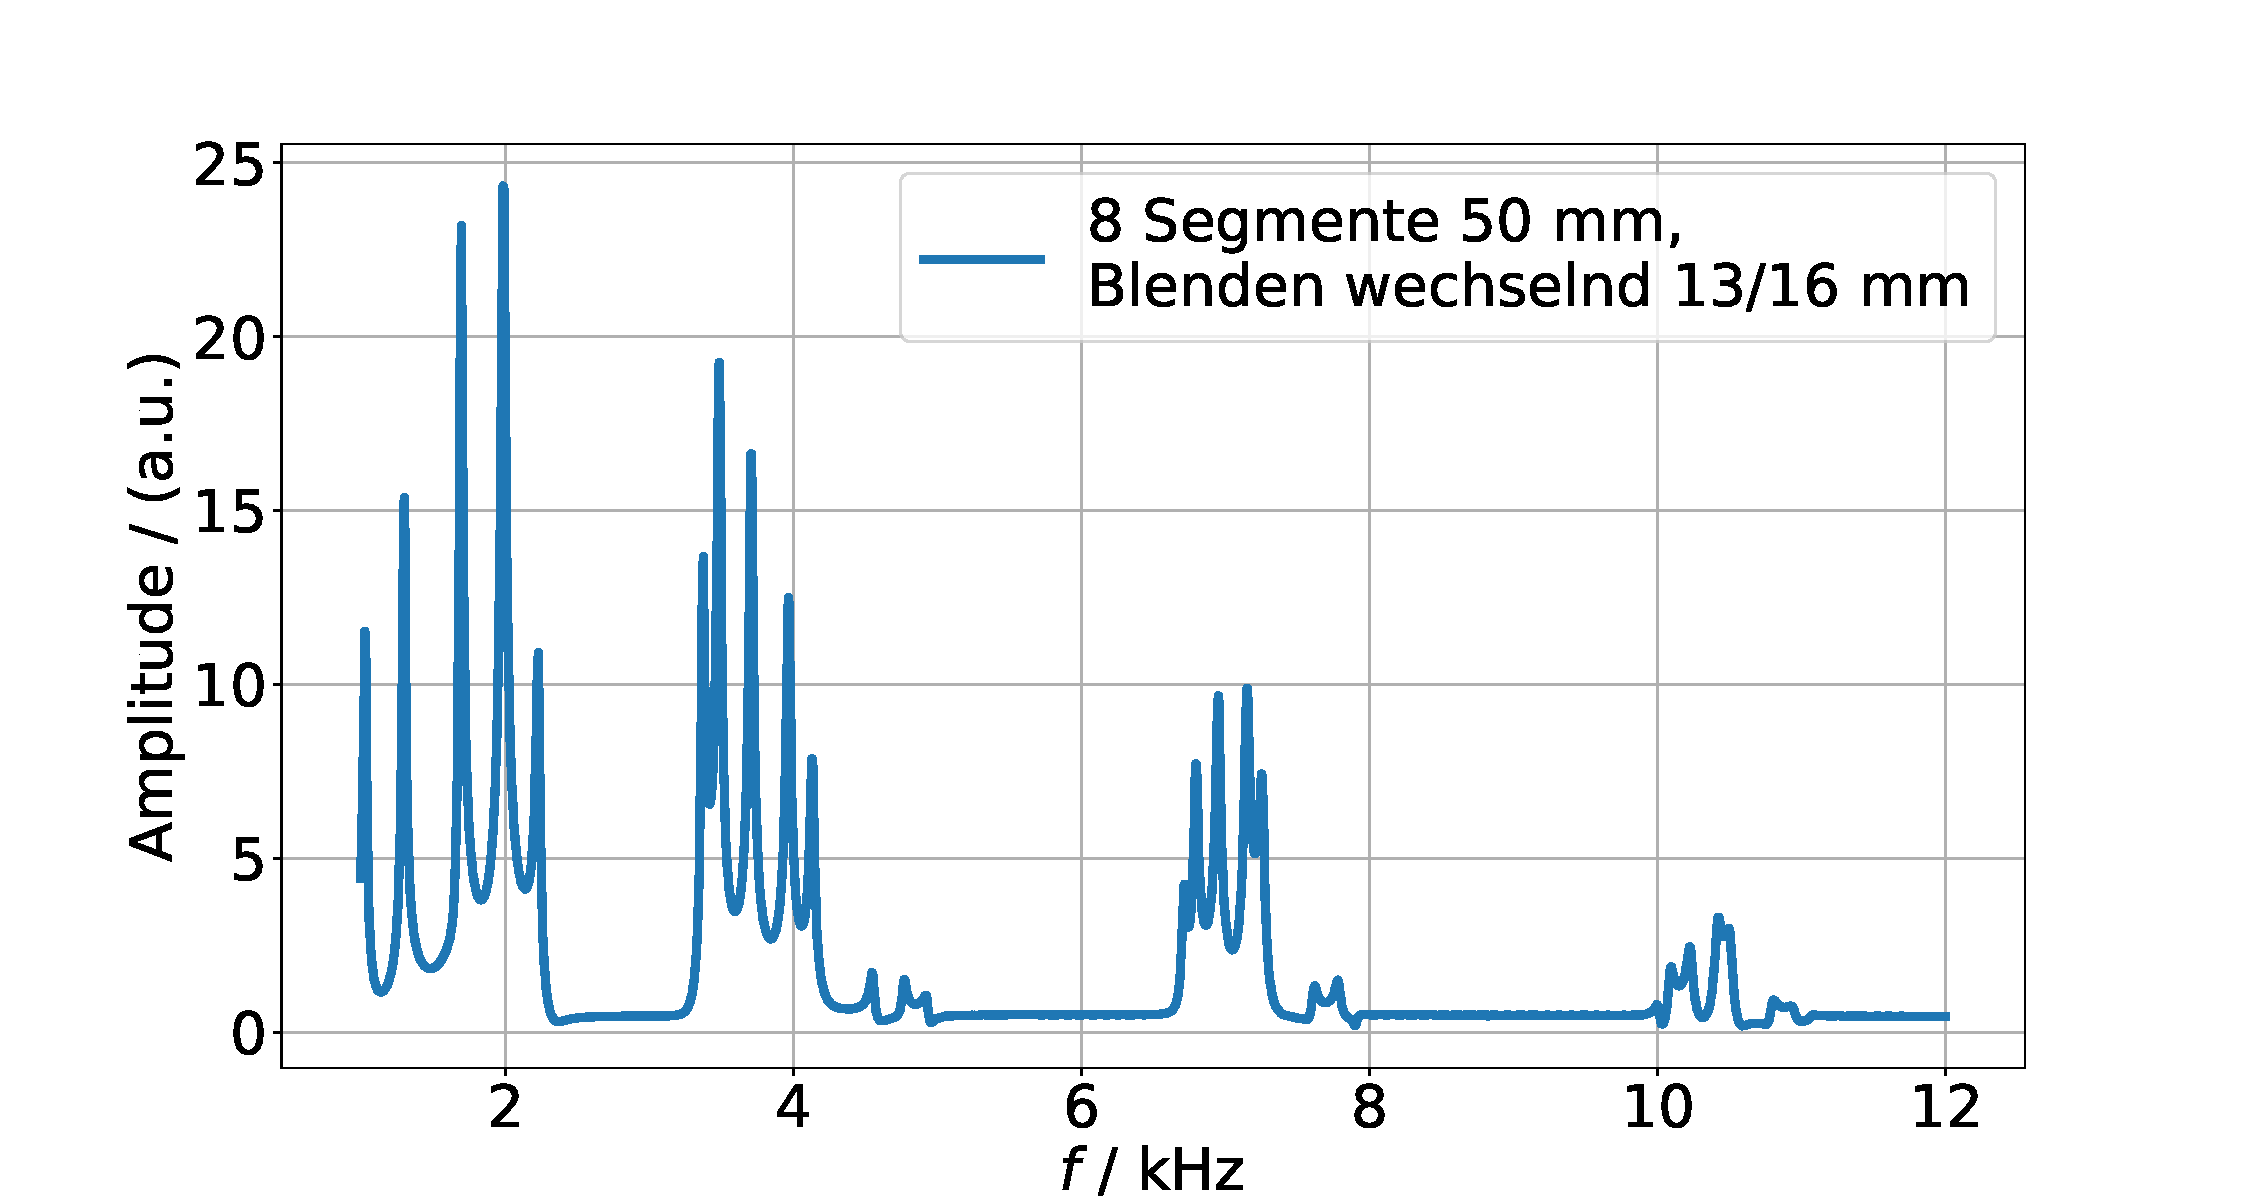
\includegraphics[width=0.8\textwidth]{plots/B_6.pdf}
    \caption{Das Frequenzspektrum für 8 Zylinder der Länge \SI{50}{\milli\metre}, zwischen die abwechselnd \SI{13}{\milli\metre} und \SI{16}{\milli\metre} Blenden gesetzt wurden.}
    \label{fig:var5}
\end{figure}

\subsection{Wasserstoffatom}

In Abb. \ref{fig:Wasserstoff1} ist das Frequenzspektrum eines Kugelresonators bei einem Winkel von $\alpha = \SI{180}{\degree}$ zwischen Lautsprecher und Mikrofon zu sehen. Dabei ist der erste Peak ein Resultat der Transferfunktion und keine Eigenschaft des Kugelresonators. 
Die Daten werden in \SI{5}{\hertz} Schritten bei \SI{60}{\milli\second} pro Schritt aufgenommen. 

\begin{figure}
    \centering
    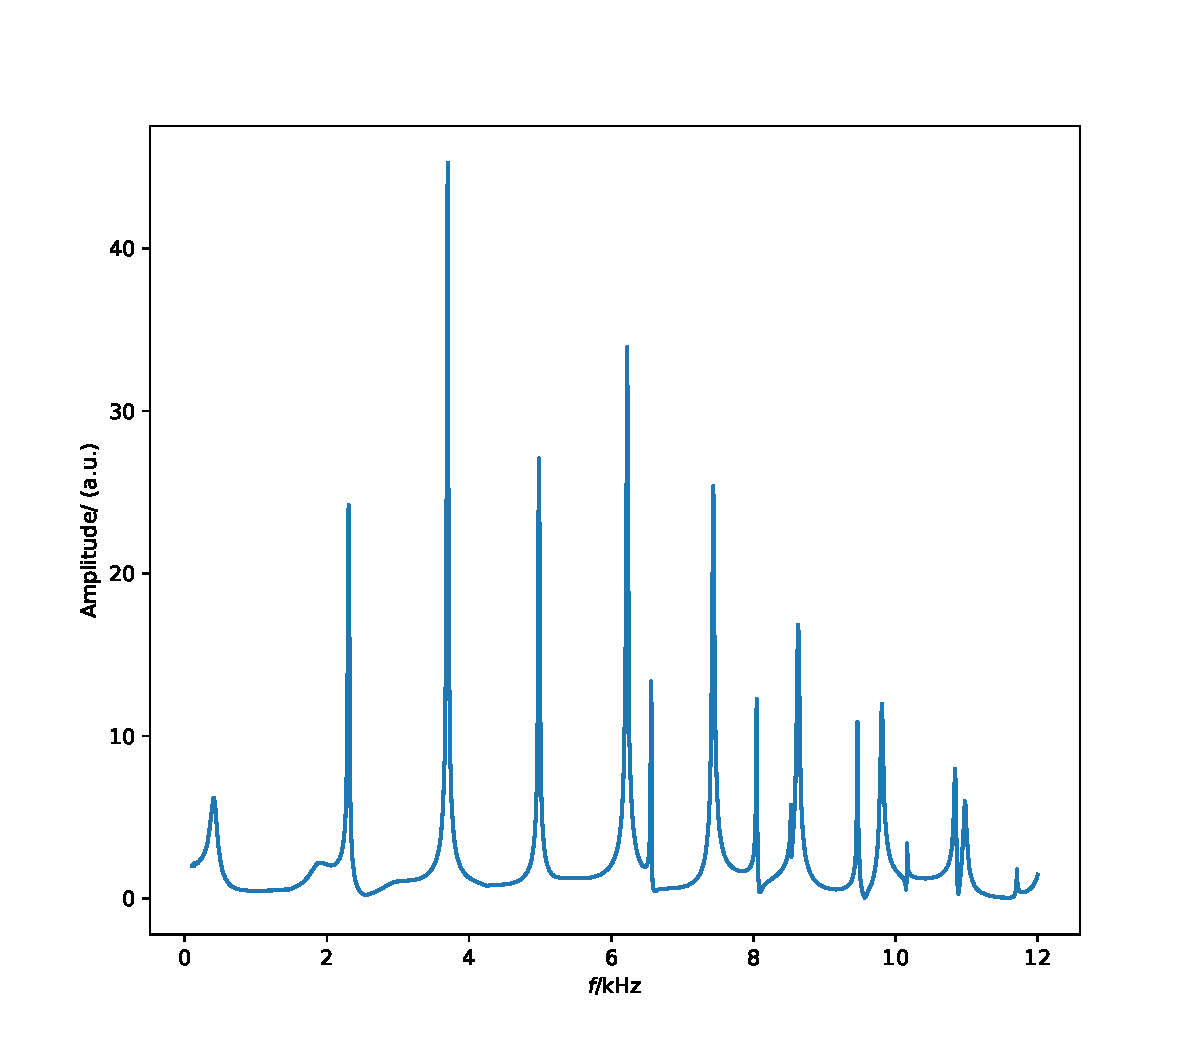
\includegraphics[width=0.8\textwidth]{plots/C_1.pdf}
    \caption{Zu sehen ist das Frequenzspektrum eines Kugelresonators bei einem eingestellten Winkel von \SI{180}{\degree}.}
    \label{fig:Wasserstoff1}
\end{figure}

Die Winkelabhängigkeit der Amplitude von den Resonanzen bei \SI{2.3}{\kilo\hertz}, \SI{3.7}{\kilo\hertz}, \SI{5}{\kilo\hertz} und bei \SI{7.4}{\kilo\hertz} wird im Folgenden untersucht. 

Dazu sind die Amplitudenwerte für alle vier Peaks bei Winkeln von \SI{90}{\degree} bis \SI{180}{\degree}, die in Tabelle \ref{tab:winkel} aufgelistet sind, als Polarplots in Abb. \ref{fig:polar23} aufgetragen und gegen die Beträge der Legendrepolynome mit einem freien Parameter für die Amplitude gefittet worden. Der geplottete Winkel ist $\theta$ und wurde nach Formel \eqref{theta} aus dem gemessenen Winkel $\alpha$ bestimmt.
Die Ergebnisse dieses Fits und die dazugehörenden Werte für $l$ und die entsprechenden Legendrepolynome sind in Tab. \ref{tab:fit} aufgelistet.

\begin{figure}
    \centering
    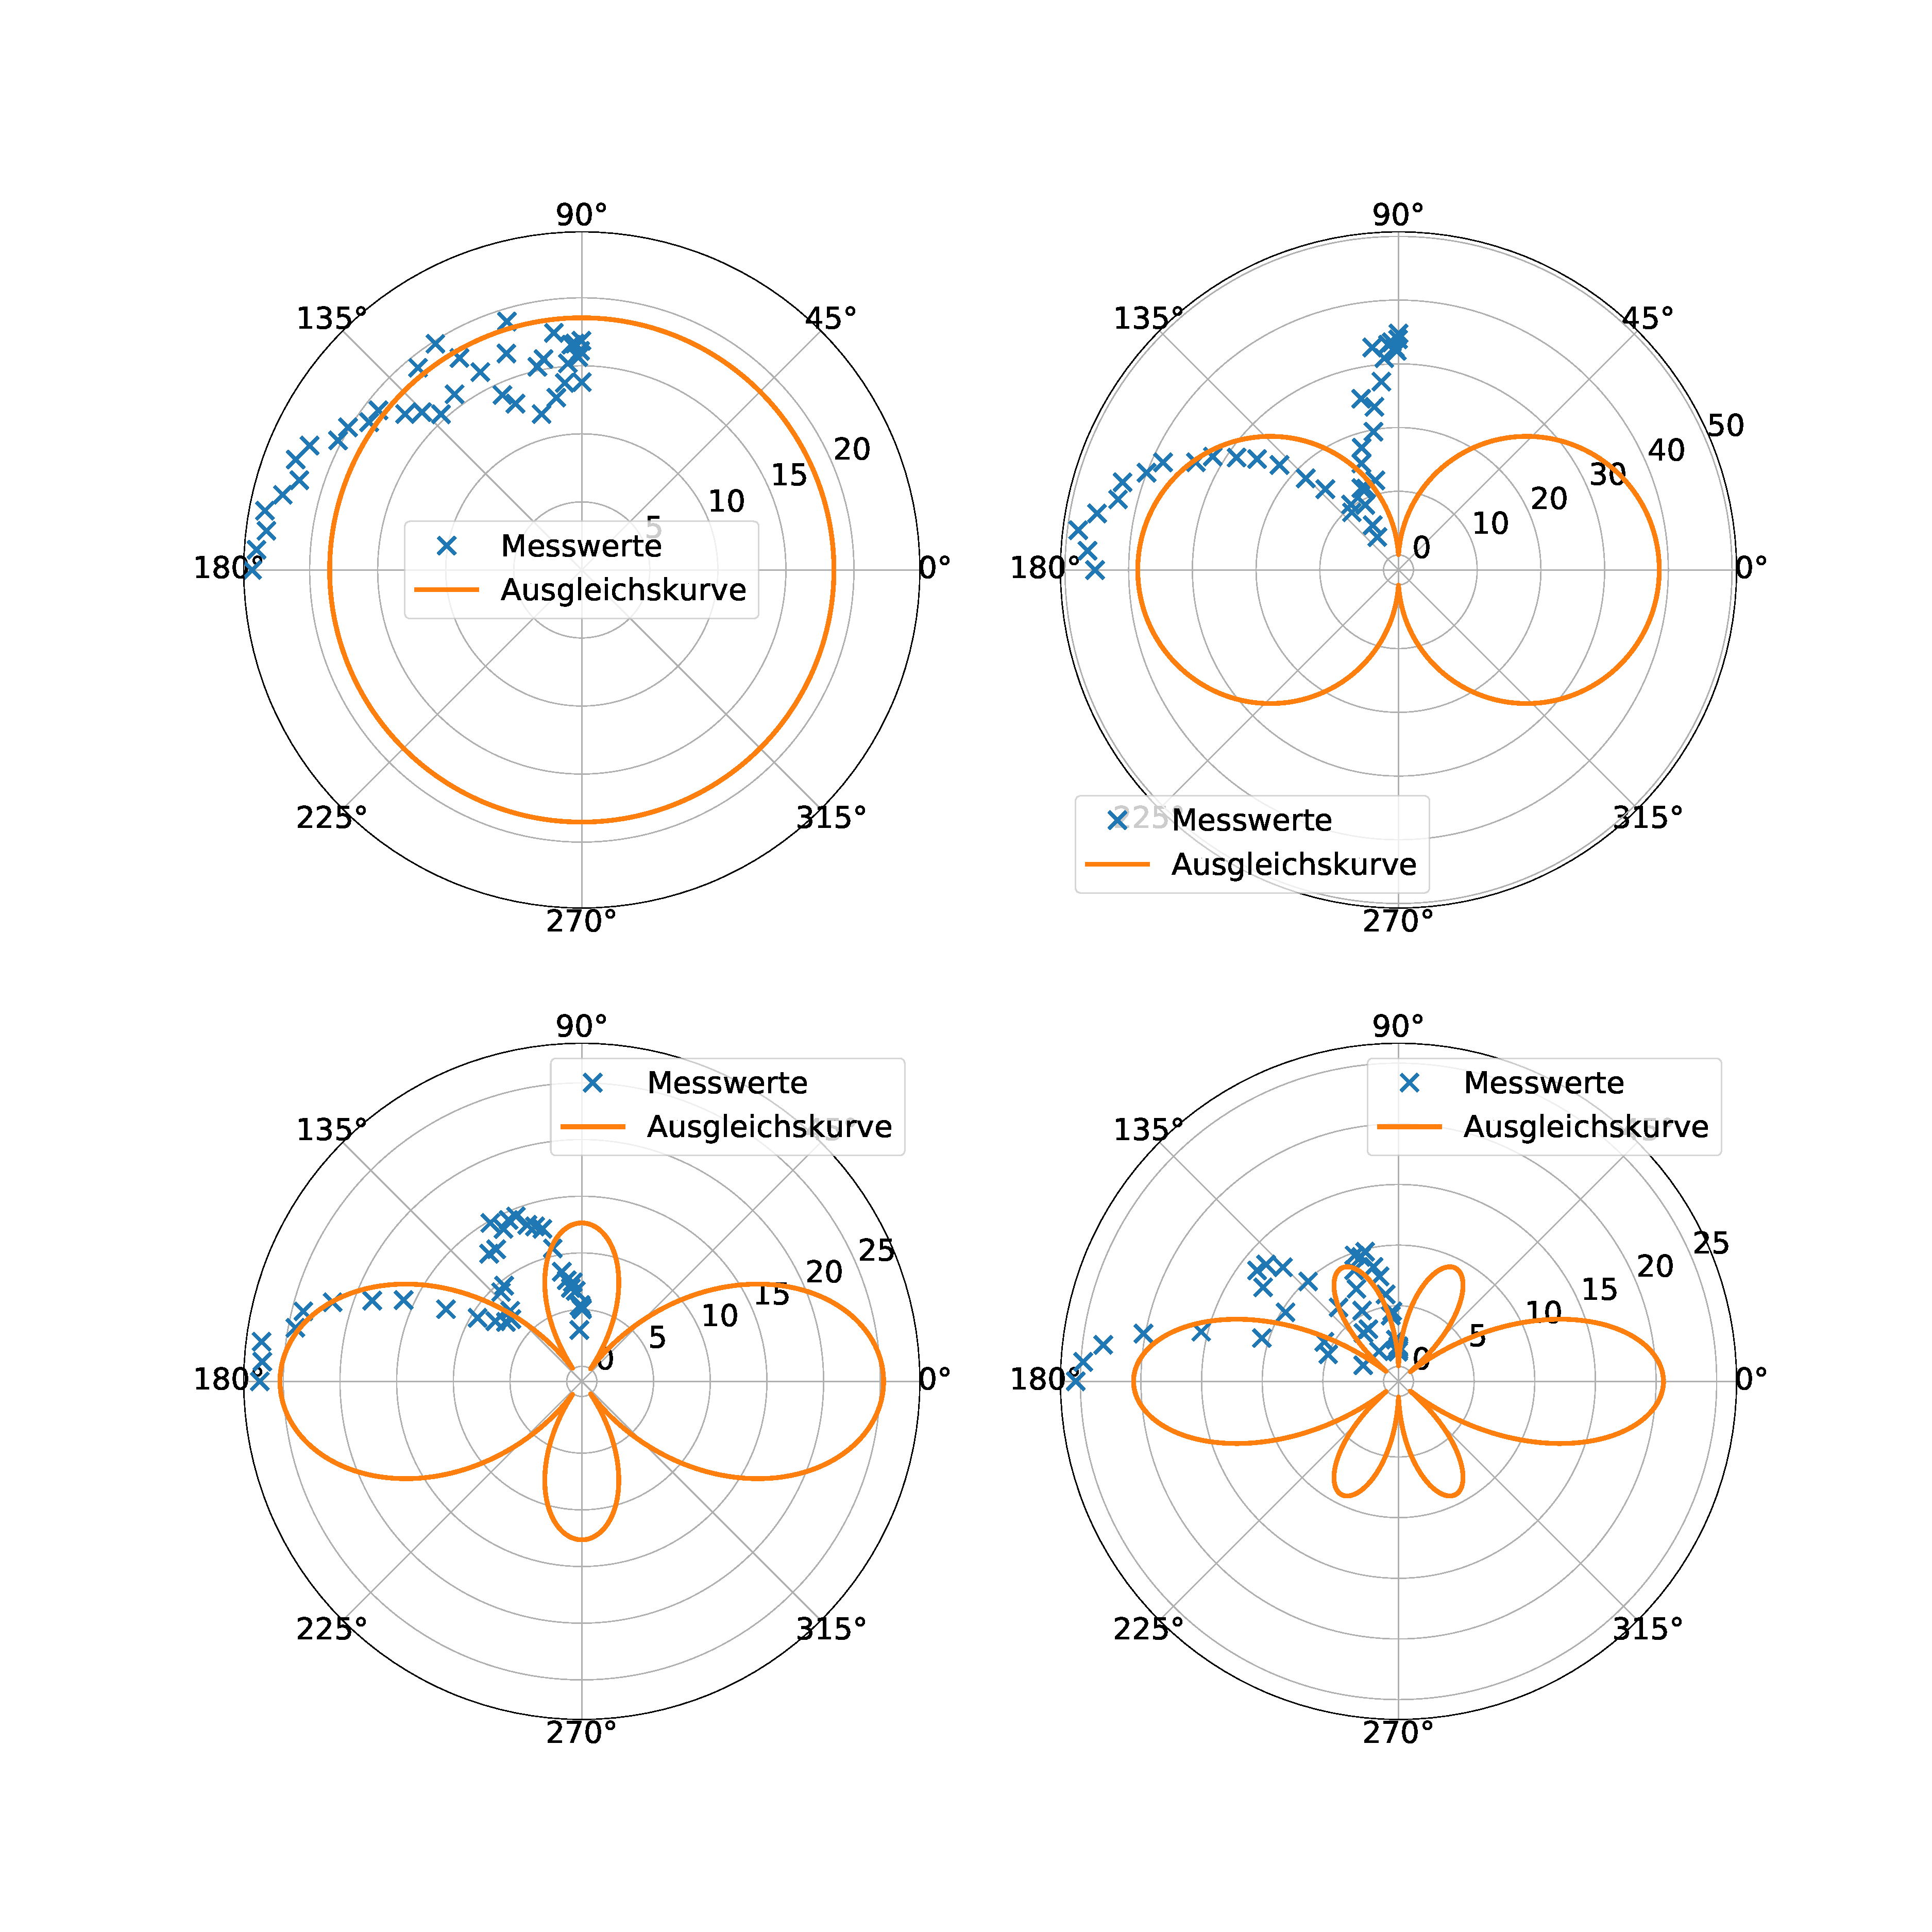
\includegraphics[width=\textwidth]{plots/C_polar1.pdf}
    \caption{Die Winkelverteilung der Amplitude bei der Resonanzfrequenz von \SI{2.3}{\kilo\hertz}, \SI{3.7}{\kilo\hertz}, \SI{5.0}{\kilo\hertz} und \SI{7.4}{\kilo\hertz} sind hier abgebildet als Polarplot. Der geplottete Winkel ist $\theta$.}
    \label{fig:polar23}
\end{figure}


\begin{table}\caption{Die Amplituden der jeweiligen Peaks bei verschiedenen Winkeln $\theta$. Der Winkel $\alpha$ wurde mit Formel \eqref{theta} in den  Winkel $\theta$ umgerechnet.}
    \label{tab:winkel}
    \centering
    \sisetup{round-mode = places, round-integer-to-decimal=true}
     \begin{tabular}{S[round-precision=1] S[round-precision=1] S[] S[] S[] S[]} 
        %\begin{tabular}{c | c c c  | c c c}  
    \toprule
    {$\alpha / \si{\degree}$} &{$\theta / \si{\degree}$} & {\SI{2.3}{\kilo\hertz}} & {\SI{3.7}{\kilo\hertz}} & {\SI{5.0}{\kilo\hertz}} & {\SI{7.4}{\kilo\hertz}} \\
\midrule
0& 90   & 13.798 & 34.743 & 1.536  & 5.016 \\
5& 90.10901394   & 16.835 & 33.836 & 1.367  & 5.181 \\
10 & 90.43523  & 16.087 & 32.049 & 1.653  & 5.142 \\
15 & 90.9762004  & 15.631 & 32.509 & 1.217  & 5.410 \\
20 & 91.72794107  & 16.645 & 33.383 & 1.281  & 5.316 \\
25 & 92.68506689  & 16.575 & 33.048 & 1.450  & 3.216 \\
30 & 93.84096572  & 15.220 & 30.944 & 2.212  & 6.671 \\
35 & 95.18799869  & 13.801 & 27.321 & 4.556  & 7.446 \\
40 & 96.71771346  & 17.534 & 32.818 & 4.233  & 6.961 \\
45 & 98.42105812  & 12.796 & 23.519 & 6.006  & 7.684 \\
50 & 100.28858514  & 15.749 & 19.691 & 7.563  & 8.498 \\
55 & 102.31063759  & 15.275 & 25.151 & 8.429  & 10.665 \\
60 & 104.47751219  & 11.834 & 12.170 & 9.797  & 12.564 \\
65 & 106.77959649  & 19.064 & 17.697 & 9.474  & 12.956 \\
70 & 109.20747973  & 16.835 & 15.371 & 9.754  & 13.297 \\
75 & 111.75203816  & 13.161 & 11.371 & 8.637  & 14.343 \\
80 & 114.40449734  & 14.115 & 11.738 & 7.145  & 14.297 \\
85 & 117.15647388  & 16.342 & 9.101  & 5.333  & 13.789 \\
90 & 120  & 17.984 & 5.767  & 3.734  & 14.805 \\
95 & 122.92753382  & 19.791 & 3.796  & 1.721  & 12.558 \\
100 & 125.93195832 & 15.938 & 10.346 & 3.692  & 12.581 \\
105 & 129.0065716 & 19.116 & 9.280  & 6.618  & 9.532 \\
110 & 132.14507056 & 15.422 & 14.740 & 9.870  & 9.287 \\
115 & 135.34152988 & 16.498 & 18.118 & 12.149 & 7.541 \\
120 & 138.59037789 & 17.315 & 22.537 & 13.324 & 6.960 \\
125 & 141.88637038 & 18.989 & 25.853 & 13.585 & 7.171 \\
130 & 145.22456333 & 19.023 & 28.578 & 12.351 & 7.949 \\
135 & 148.60028519 & 20.117 & 31.793 & 9.682  & 9.438 \\
140 & 152.00910928 & 20.280 & 33.668 & 5.700  & 12.237 \\
145 & 155.44682653 & 21.994 & 38.268 & 1.959  & 15.939 \\
150 & 158.90941882 & 22.534 & 40.035 & 4.979  & 18.469 \\
155 & 162.39303301 & 21.777 & 43.084 & 10.581 & 21.722 \\
160 & 165.89395574 & 22.653 & 43.045 & 15.539 & 23.990 \\
165 & 169.40858887 & 23.685 & 45.776 & 20.151 & 24.376 \\
170 & 172.93342561 & 23.354 & 48.303 & 23.292 & 27.137 \\
175 & 176.46502721 & 23.948 & 46.561 & 24.815 & 26.895 \\
180 & 180 & 24.225 & 45.271 & 25.372 & 27.076 \\

\bottomrule
\end{tabular}\end{table}



\begin{table}\caption{Die Ergebnisse der Ausgleichsrechnung zu den Beträgen der Legendrepolynome. In allen vier Fällen ist $m = 0$.}
    \label{tab:fit}
    \centering
    \sisetup{round-mode = places, round-integer-to-decimal=true}
     \begin{tabular}{c c S[round-precision=1] c} 
        %\begin{tabular}{c | c c c  | c c c}  
    \toprule
{$f / \si{\kilo\hertz}$} & {$l$} & {Amplitudenwert} & Legendrepolynom $P_l^m$ \\
\midrule
2,7     &   1   &  25.9(15)  &   $\cos \theta$   \\
3,7     &   2   &  49.7(13) &   $\frac{1}{2}(3 \cos(\theta)^2 -1)$ \\
5,0     &   3   &  29.7(8) &   $\frac{1}{2} (5  \cos(\theta)^3 -3 \cos(\theta))$  \\ 
7,4     &   5   &  27.2(5) &   $\frac{1}{8} (63  \cos(\theta)^5 -70 \cos(\theta)^3 + 15\cos(\theta))$  \\

\bottomrule
\end{tabular}\end{table}

Der Peak bei ca. \SI{2.3}{\kilo\hertz} wird mit verschiedenen Zwischenringen überprüft.
Die Aufspaltung der drei Peaks ist in Tabelle \ref{tab:aufspaltung} gegen die Dicke der Ringe aufgelistet und in Abb. \ref{fig:aufspaltung} aufgetragen.

\begin{table}\caption{Die Aufspaltung der Peaks ist gegen die Dicke des Zwischenrings aufgelistet.}
    \label{tab:aufspaltung}
    \centering
    \sisetup{round-mode = places, round-integer-to-decimal=true}
     \begin{tabular}{c c S[round-precision=1] c} 
        %\begin{tabular}{c | c c c  | c c c}  
    \toprule
{Ringdicke / \si{\milli\metre}} & {Aufspaltung / \si{\hertz}}  \\
\midrule
0 & 0 \\
3 & 63 \\
6 & 111 \\
9 & 173 \\
\bottomrule
\end{tabular}\end{table}

\begin{figure}
    \centering
    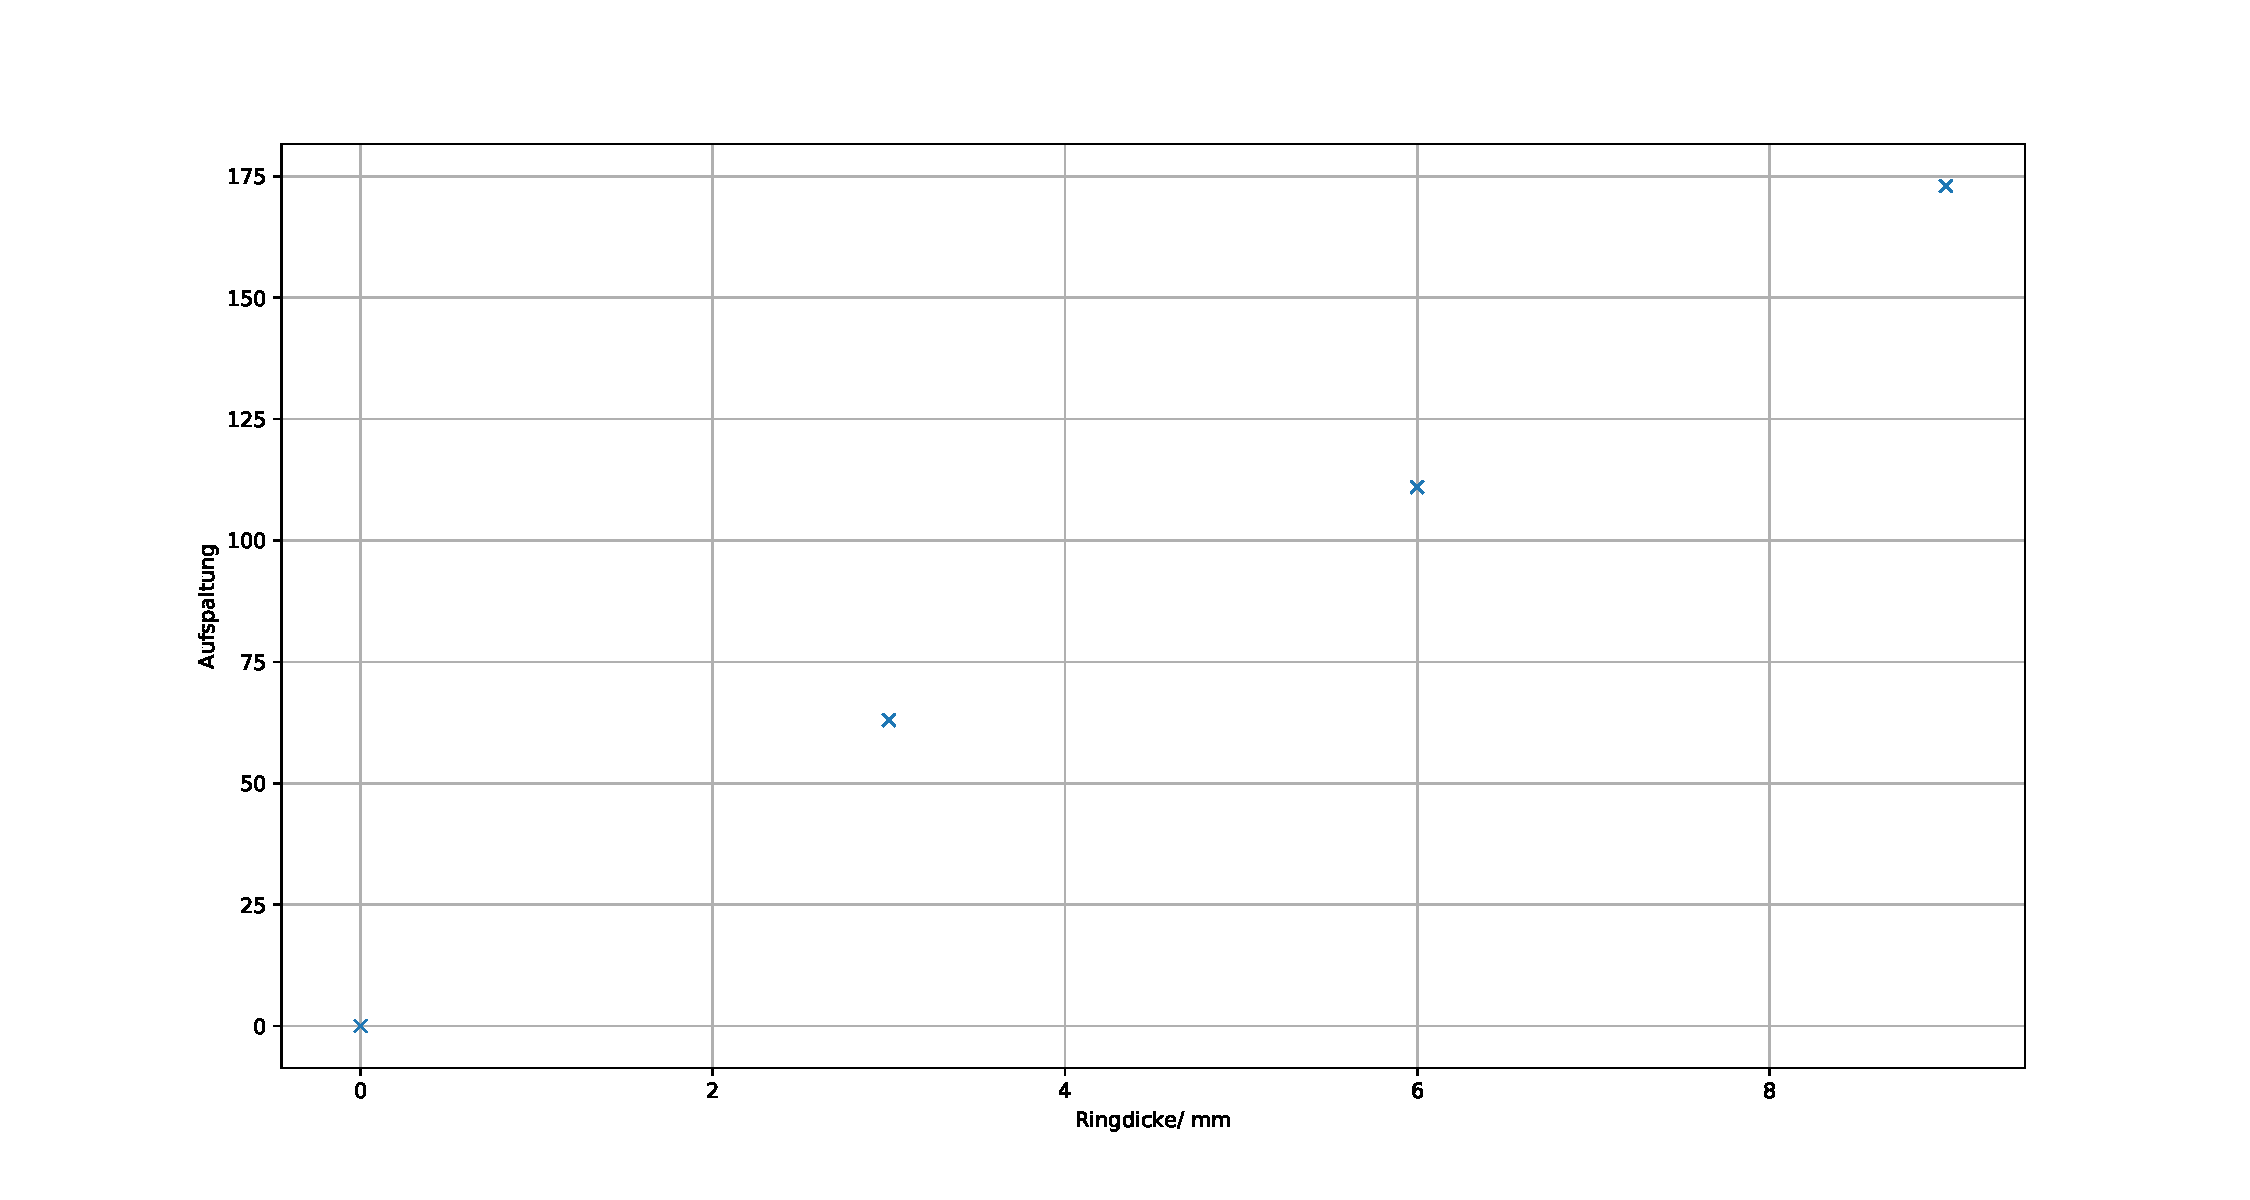
\includegraphics[width=0.8\textwidth]{plots/C_Aufspaltung.pdf}
    \caption{Die Aufspaltung des Peaks ist gegen die Dicke des Zwischenrings aufgetragen. Die einzelnen Datenpunkte sind eingetragen.}
    \label{fig:aufspaltung}
\end{figure}

Mit einer Dicke des Rings von \SI{9}{\milli\meter} wird die Winkelabhängigkeit der Amplitude erneut überprüft. Die Ergebnisse liegen in Tabelle \ref{tab:winkel2}
In Abb. \ref{fig:polar2} ist diese in einem Polarplot aufgetragen. Die dazugehörigen Quantenzahlen sind $l=1$ und $m=0$ bzw. $l=1$ und $m = 1$. 
Die Symmetriebrechung führt dazu, dass das Polynom $P^0_1$ bei einer Frequenz von \SI{2.1}{\kilo\hertz} mit einer Amplitude von \num{13.41(7)} zu finden ist, während das Legendrepolynom $P^1_1$ bei einer Frequenz von \SI{2.27}{\kilo\hertz} und einer Amplitude von \num{24.40(13)} vorliegt, während $P^0_1$ vorher bei \SI{2.3}{\kilo\hertz} lag. %so richtig?

\begin{table}\caption{Die Amplituden der jeweiligen Peaks bei verschiedenen Winkeln.}
    \label{tab:winkel2}
    \centering
    \sisetup{round-mode = places, round-integer-to-decimal=true}
     \begin{tabular}{S[round-precision=1] S[] S[] | S[round-precision=1] S[] S[]} 
        %\begin{tabular}{c | c c c  | c c c}  
    \toprule
{$\phi / \si{\degree}$} & {\SI{2.1}{\kilo\hertz}} & {\SI{2.27}{\kilo\hertz}} & {$\phi / \si{\degree}$} & {\SI{2.1}{\kilo\hertz}} & {\SI{2.27}{\kilo\hertz}} \\
\midrule
  
5 & 13.438 & 25.133 &      95    & 1.528 & 24.112  \\
10     & 13.379 & 25.267&  100    & 2.597 & 24.289  \\
15    & 13.237 & 25.199 &  105 & 3.559 & 24.357 \\
20   & 12.954 & 25.388 &   110  & 4.564 & 24.383 \\
25   & 12.614 & 25.085 &   115  & 5.693 & 24.140 \\
30   & 12.050 & 24.969 &   120  & 6.786 & 24.170 \\
35   & 11.515 & 25.046 &   125  & 7.590 & 24.058 \\
40   & 10.706 & 25.046 &   130  & 8.444 & 24.149 \\
45   & 9.939 & 25.033 &    135  & 9.270 & 24.177 \\
50  & 8.946 & 24.944  &    140  & 9.964 & 24.175  \\
55  & 8.153 & 24.952  &    145  & 10.660 & 24.780  \\
60  & 6.929 & 24.913  &    150  & 11.344 & 23.992  \\
65  & 5.828 & 24.776  &    155  & 11.906 & 24.902  \\
70  & 4.543 & 24.738  &    160  & 12.130 & 23.916  \\
75  & 3.101 & 23.999  &    165  & 12.527 & 23.812  \\
80  & 2.142 & 24.166  &    170  & 12.878 & 22.127  \\
85  & 1.003 & 24.359  &    175  & 12.794 & 22.406  \\
90  & 0.438 & 24.428  &    180  & 13.427 & 25.182  \\
\bottomrule
\end{tabular}\end{table}


\begin{figure}
    \centering
    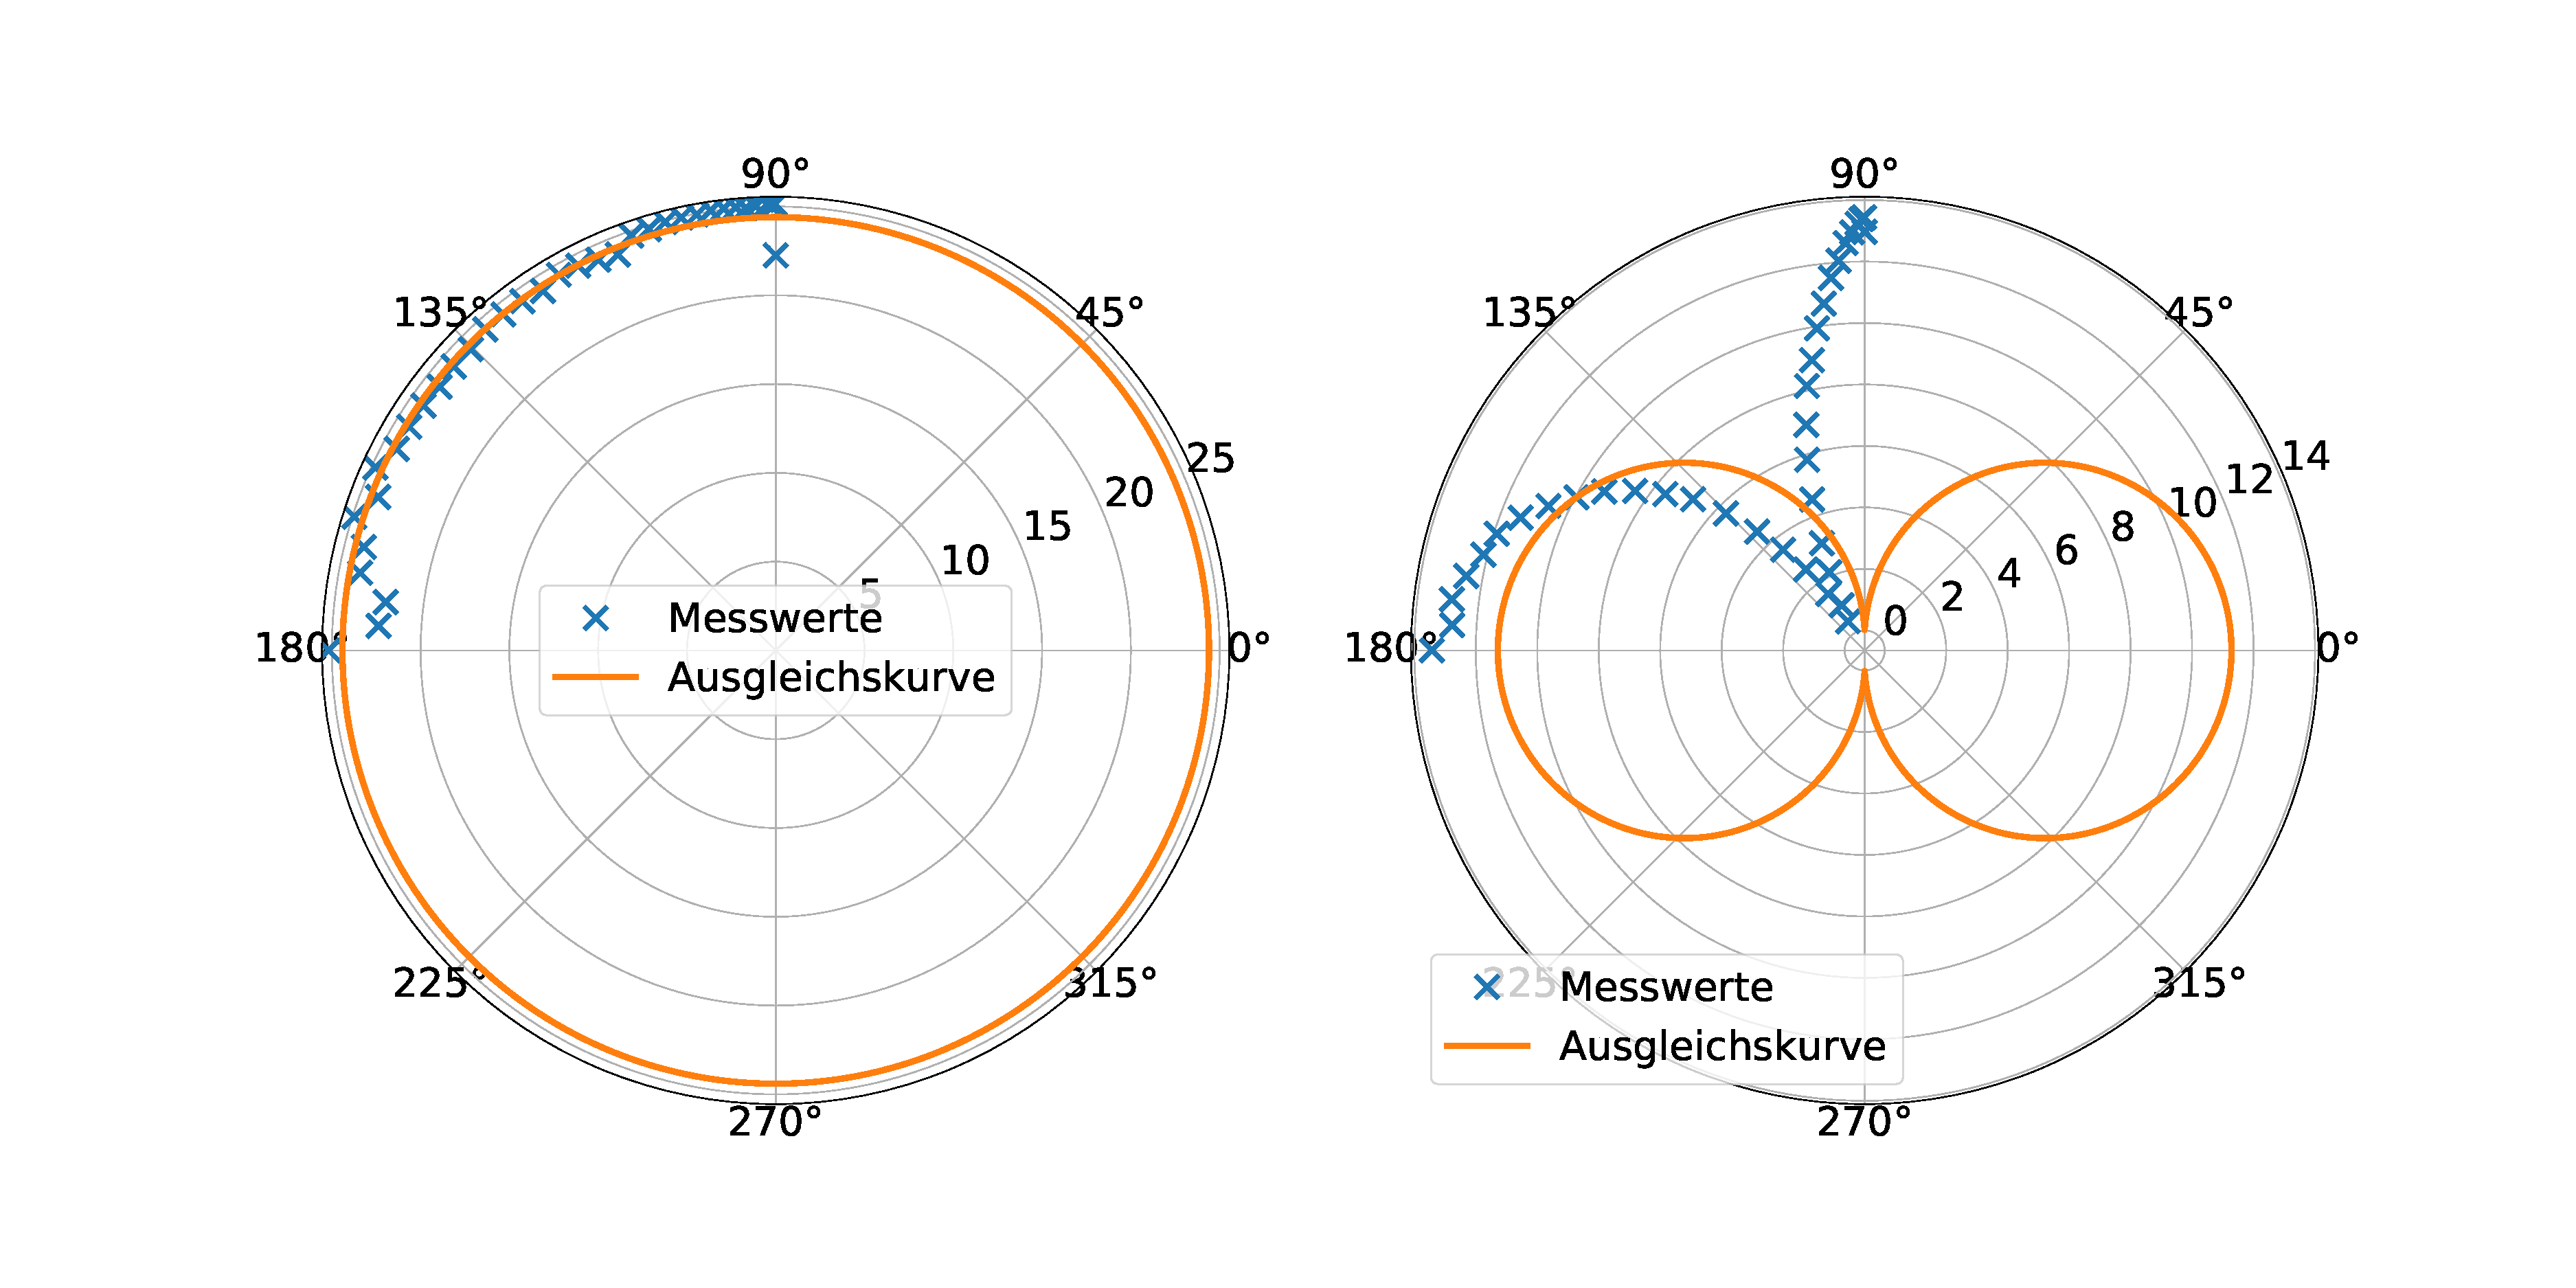
\includegraphics[width=0.85\textwidth]{plots/C_polar5.pdf}
    \caption{Die Winkelverteilung der Amplitude bei der Resonanzfrequenz von \SI{2.1}{\kilo\hertz} und \SI{2.27}{\kilo\hertz} mit einem Zwischenring der Dicke \SI{9}{\milli\metre}.}
    \label{fig:polar2}
\end{figure}

\subsection{Wasserstoffmolekül}

Zur Darstellung eines Wasserstoffmoleküls werden zwei Kugelresonatoren, die durch ein Loch verbunden sind, übereinandergesetzt.
Das Frequenzspektrum für den Resonator ohne Blende und mit drei verschiedenen Blenden ist in Abb. \ref{fig:molek1} zu sehen.

\begin{figure}
    \centering
    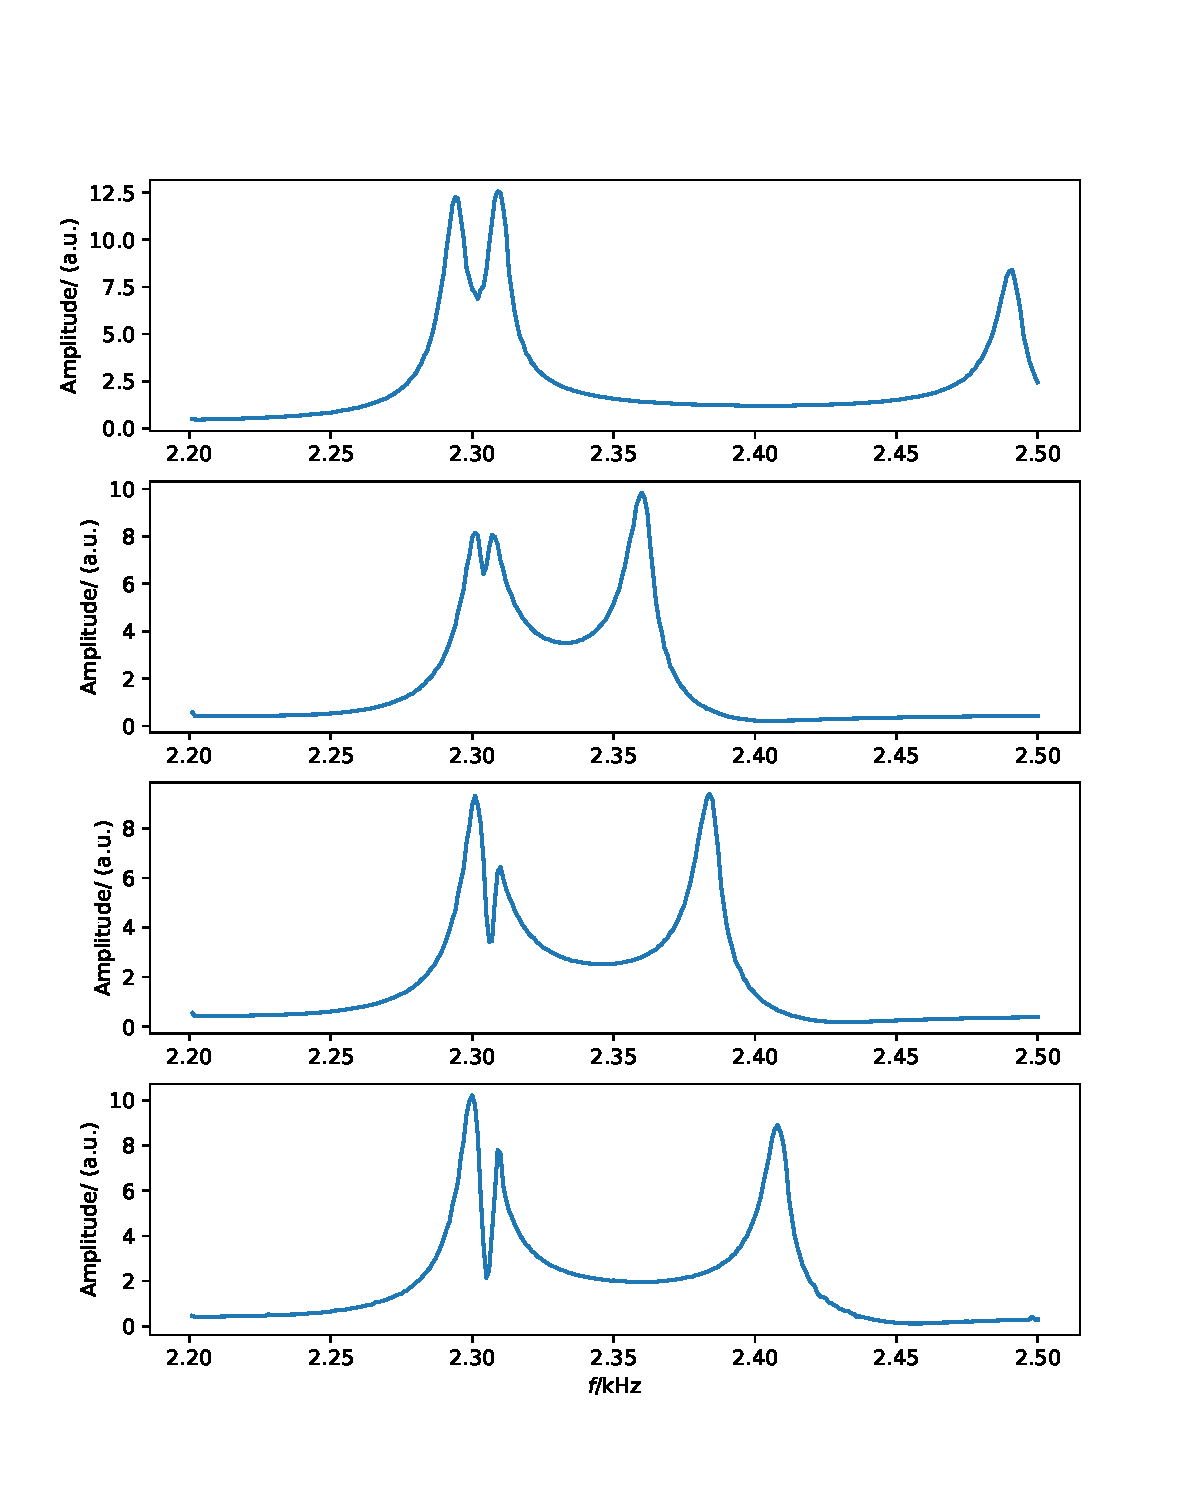
\includegraphics[height=0.7\textheight]{plots/D_1.pdf}
    \caption{Das Spektrum für den Resonator ohne Blende. Darunter ist das Spektrum für den Resonator mit einer Blende von \SI{10}{\milli\metre}, \SI{13}{\milli\metre} und \SI{16}{\milli\metre} Durchmesser.}
    \label{fig:molek1}
\end{figure}

In Abb. \ref{fig:resonanzen} ist die Resonanzfrequenz in Abhängigkeit vom Blendendurchmesser aufgetragen. Die Werte sind in Tabelle \ref{tab:ende} aufgelistet.

\begin{table}\caption{Die resonante Frequenz der Peaks ist gegen den Durchmesser der Blende aufgelistet.}
    \label{tab:ende}
    \centering
    \sisetup{round-mode = places, round-integer-to-decimal=true}
     \begin{tabular}{c | c c c} 
        %\begin{tabular}{c | c c c  | c c c}  
    \toprule
{Blendendurchmesser / \si{\milli\meter}} & {Peak 1} & {Peak 2} & {Peak 3}   \\
\midrule
-  & 2294.0 & 2294.0 & 2309.0 \\ 
10 & 2301.0 & 2307.0 & 2360.0 \\
13 & 2301.0 & 2310.0 & 2384.0 \\
16 & 2300.0 & 2309.0 & 2408.0 \\
\bottomrule
\end{tabular}\end{table}

\begin{figure}
    \centering
    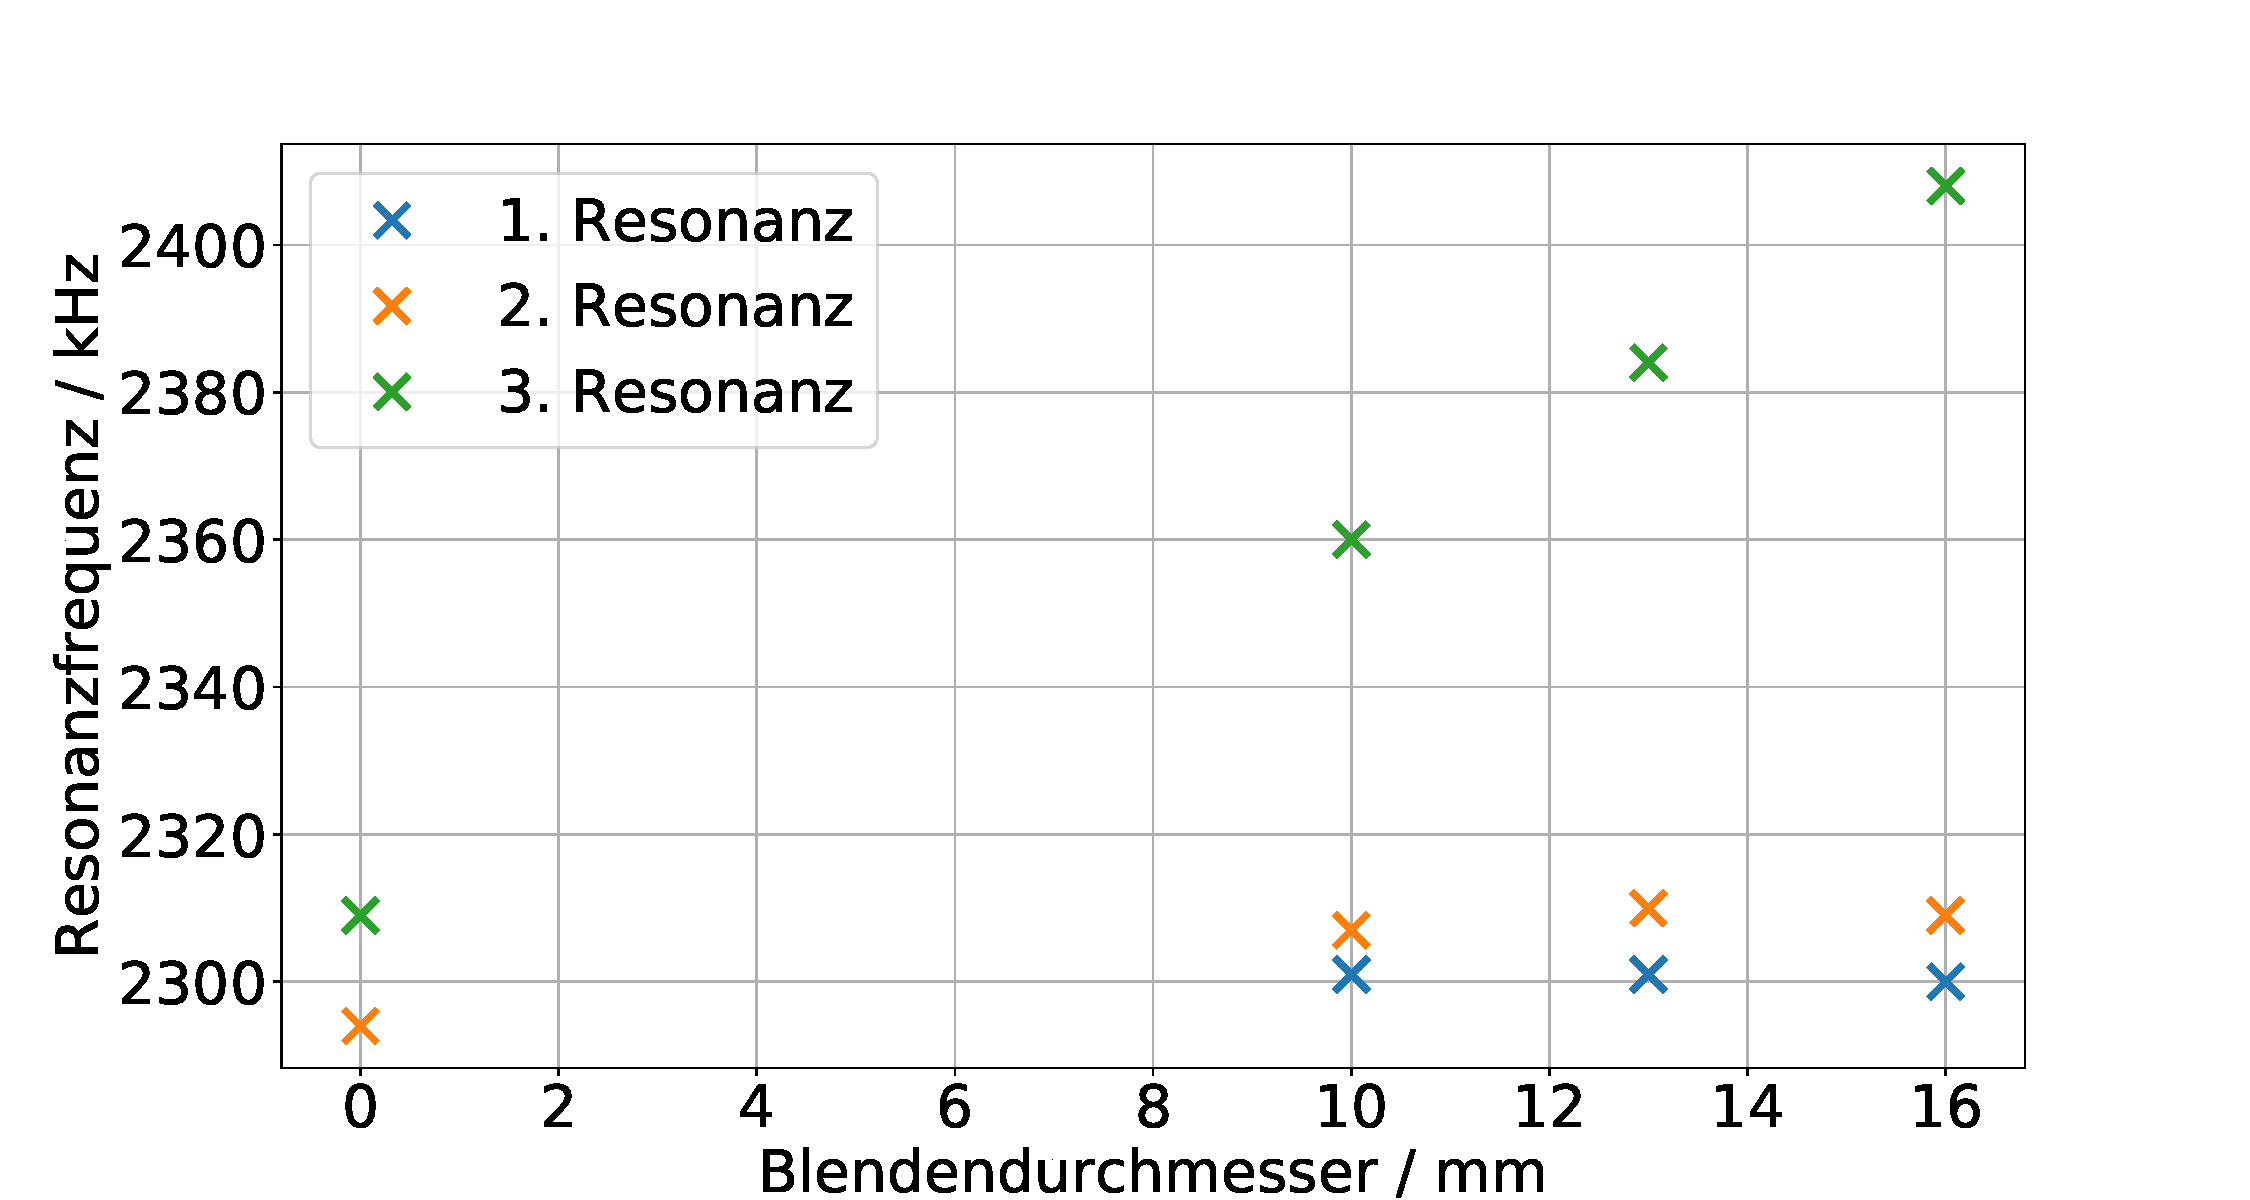
\includegraphics[width=0.8\textwidth]{plots/D_2.pdf}
    \caption{Die resonante Frequenz der Peaks ist gegen den Durchmesser der Blende aufgelistet.}
    \label{fig:resonanzen}
\end{figure}

Das Frequenzspektrum mit einer Blende mit Durchmesser von \SI{16}{\milli\metre} wurde für verschiedene Winkel aufgenommen. Die Werte der Amplituden der Resonanzen bei dem jeweiligem Winkel stehen in Tab. \ref{tab:winkel2}. Die Winkelverteilung der Amplitude ist in Abb. \ref{fig:polar_molekuel} als Polarplot dargestellt. 

\begin{table}\caption{Die Amplituden der jeweiligen Peaks bei verschiedenen Winkeln $\phi$.}
    \label{tab:winkel2}
    \centering
    \sisetup{round-mode = places, round-integer-to-decimal=true}
    \begin{tabular}{S[round-precision=1] S[] S[] S[] | S[round-precision=1] S[] S[] S[]} 
    \toprule
    {$\phi / \si{\degree}$} & {\SI{2.3}{\kilo\hertz}} & {\SI{2.307}{\kilo\hertz}} & {\SI{2.409}{\kilo\hertz}} & {$\phi / \si{\degree}$} & {\SI{2.3}{\kilo\hertz}} & {\SI{2.307}{\kilo\hertz}} & {\SI{2.409}{\kilo\hertz}} \\
\midrule
0 & 10.969 & 7.359 & 9.032  &    90 & 10.76 & 5.511 & 8.97 \\
5 & 10.518 & 7.088 & 8.99   &    95 & 10.965 & 5.663 & 8.937 \\
10 & 10.648 & 7.285 & 9.058 &   100 & 10.63 & 5.891 & 9.044 \\
15 & 10.385 & 6.917 & 9.018 &   105 & 11.005 & 5.818 & 8.982 \\
20 & 10.546 & 7.092 & 9.026 &   110 & 10.735 & 6.052 & 9.06 \\
25 & 10.59 & 6.973 & 9.024  &   115 & 10.355 & 6.333 & 9.038 \\
30 & 10.517 & 7.168 & 8.995 &   120 & 10.522 & 6.3 & 8.994 \\
35 & 10.412 & 6.895 & 8.917 &   125 & 11.347 & 5.712 & 8.958 \\
40 & 10.608 & 6.768 & 9.02  &   130 & 11.37 & 5.893 & 8.97 \\
45 & 10.618 & 6.647 & 8.991 &   135 & 11.448 & 6.033 & 8.949 \\
50 & 10.423 & 5.987 & 8.997 &   140 & 10.102 & 7.361 & 8.935 \\
55 & 10.487 & 6.171 & 8.987 &   145 & 10.5 & 7.051 & 8.881 \\
60 & 10.51 & 5.403 & 8.992  &   150 & 11.599 & 6.183 & 8.916 \\
65 & 11.34 & 5.742 & 8.978  &   155 & 11.566 & 6.552 & 8.906 \\
70 & 10.374 & 5.07 & 9.009  &   160 & 11.671 & 6.155 & 8.926 \\
75 & 10.584 & 5.197 & 9.055 &   165 & 9.883 & 8.028 & 8.982 \\
80 & 10.514 & 5.311 & 9.005 &   170 & 11.447 & 6.481 & 8.904 \\
85 & 10.497 & 5.67 & 8.975  &   175 & 11.491 & 6.514 & 8.932 \\
   &        &      &        &   180 & 11.284 & 6.907 & 8.914 \\
\bottomrule
\end{tabular}\end{table}

Analog zu den $\phi$-abhängigen Messungen im Wasserstoffatom-Abschnitt deuten die dargestellten Abbildungen auf die Zustände $2 \sigma^{(*)}$ in den linken Plots mit $m = 0$ hin und der rechte Plot lässt die $1 \pi^{(*)}$ Verbindung vermuten aufgrund der Ähnlichkeit zu dem $m=1$ Plot aus dem vorherigen Abschnitt. Eine Aussage über $l$ kann zwar nicht explizit getroffen werden, aber aufgrund der Frequenzen und somit der Energien, ist diese Einschätzung der Verbindungen gut begründet. Die $1 \pi$-Zustände lassen sich leider nicht differenzieren. Auffällig ist nur, dass bei ca. \SI{70}{\degree} der Peak von \SI{2307}{\hertz} zu \SI{2311}{\hertz} gesprungen ist. Wichtig ist noch zu sagen, dass die Werte bei $\pi$-Zuständen  mit einem Wert von $\num {5}\, \mathrm{a.u.}$ subtrahiert wurden um den Background von dem \SI{2.3}{\kilo\hertz} Peak zu unterdrücken. Allgemein wäre das exakte Verfahren eine Gauß- (oder aufgrund der Antisymmetrie des Peaks eine doppelseitige Crystalball) Funktion als Fit durch die Werte zu legen, um tatsächlich den Background zu filtern, aber dies würde den Rahmen dieses Protokolls sprengen. Insofern wurde hier ein loser Schnitt gewählt, um möglichst viel Background zu separieren ohne Signal zu verlieren. 

\begin{figure}
    \centering
    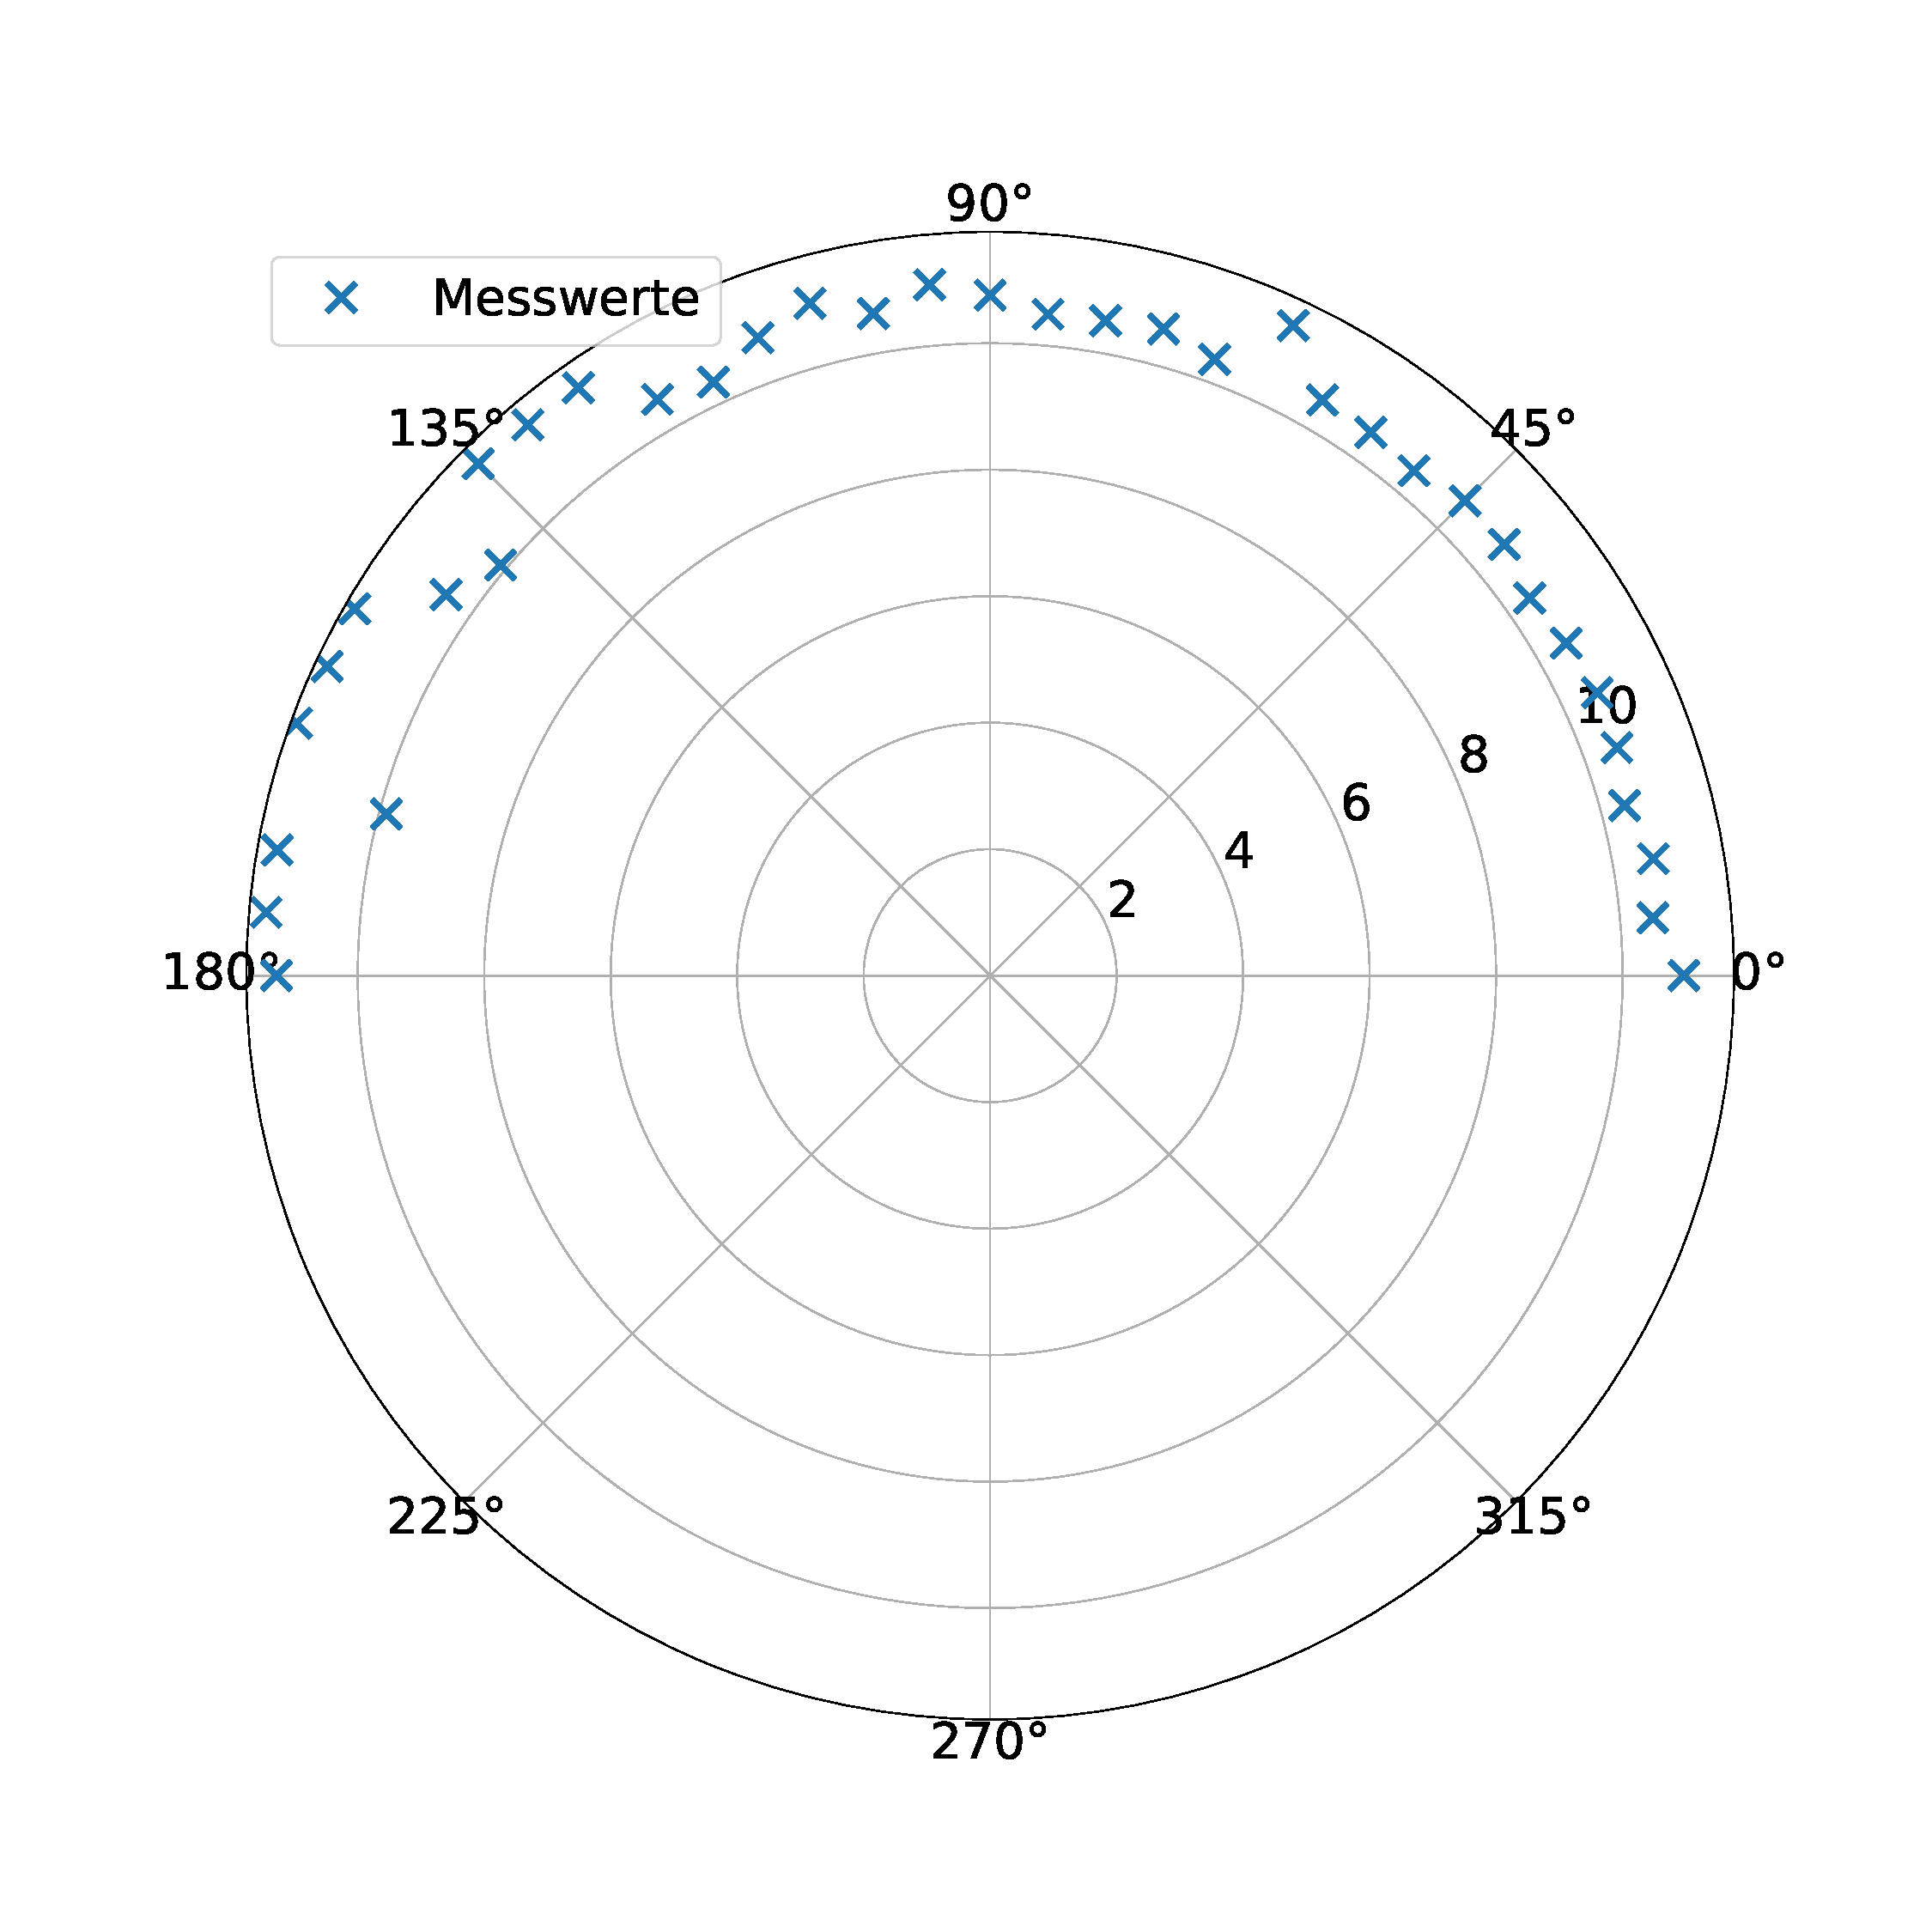
\includegraphics[width=\textwidth]{plots/D_3.pdf}
    \caption{Die Winkelverteilung der Amplitude bei der Resonanzfrequenz von \SI{2.3}{\kilo\hertz} mit einer Blende von \SI{16}{\milli\metre}. Rechts daneben ist die Winkelverteilung der Amplitude bei \SI{2.307}{\kilo\hertz} zu sehen, unten die bei \SI{2.409}{\kilo\hertz}. Der Winkel $\phi$ wurde vermessen. Bei der Amplitude bei der Resonanzfrequenz von \SI{2.307}{\kilo\hertz} ist jeweils die Amplitude bei \SI{90}{\degree} abgezogen worden.}
    \label{fig:polar_molekuel}
\end{figure}

   
In Abb. \ref{fig:phase} wurde die obere und die untere Kugel bei dem gleichen Winkel $\alpha=\SI{180}{\degree}$ gemessen. 
Nicht alle vier Peaks sind zu erkennen. Der zweite Peak bei \SI{2.3}{\kilo\hertz} fehlt in dieser Darstellung bei der oberen Kugel. Bei der unteren Kugel fehlt sogar die Aufspaltung der oberen Kugel, was unerwartet ist. Messungen mit dem Oszilloskop hätten Erkenntnisse bezüglich der Phasenverschiebung gebracht. 

\begin{figure}
    \centering
    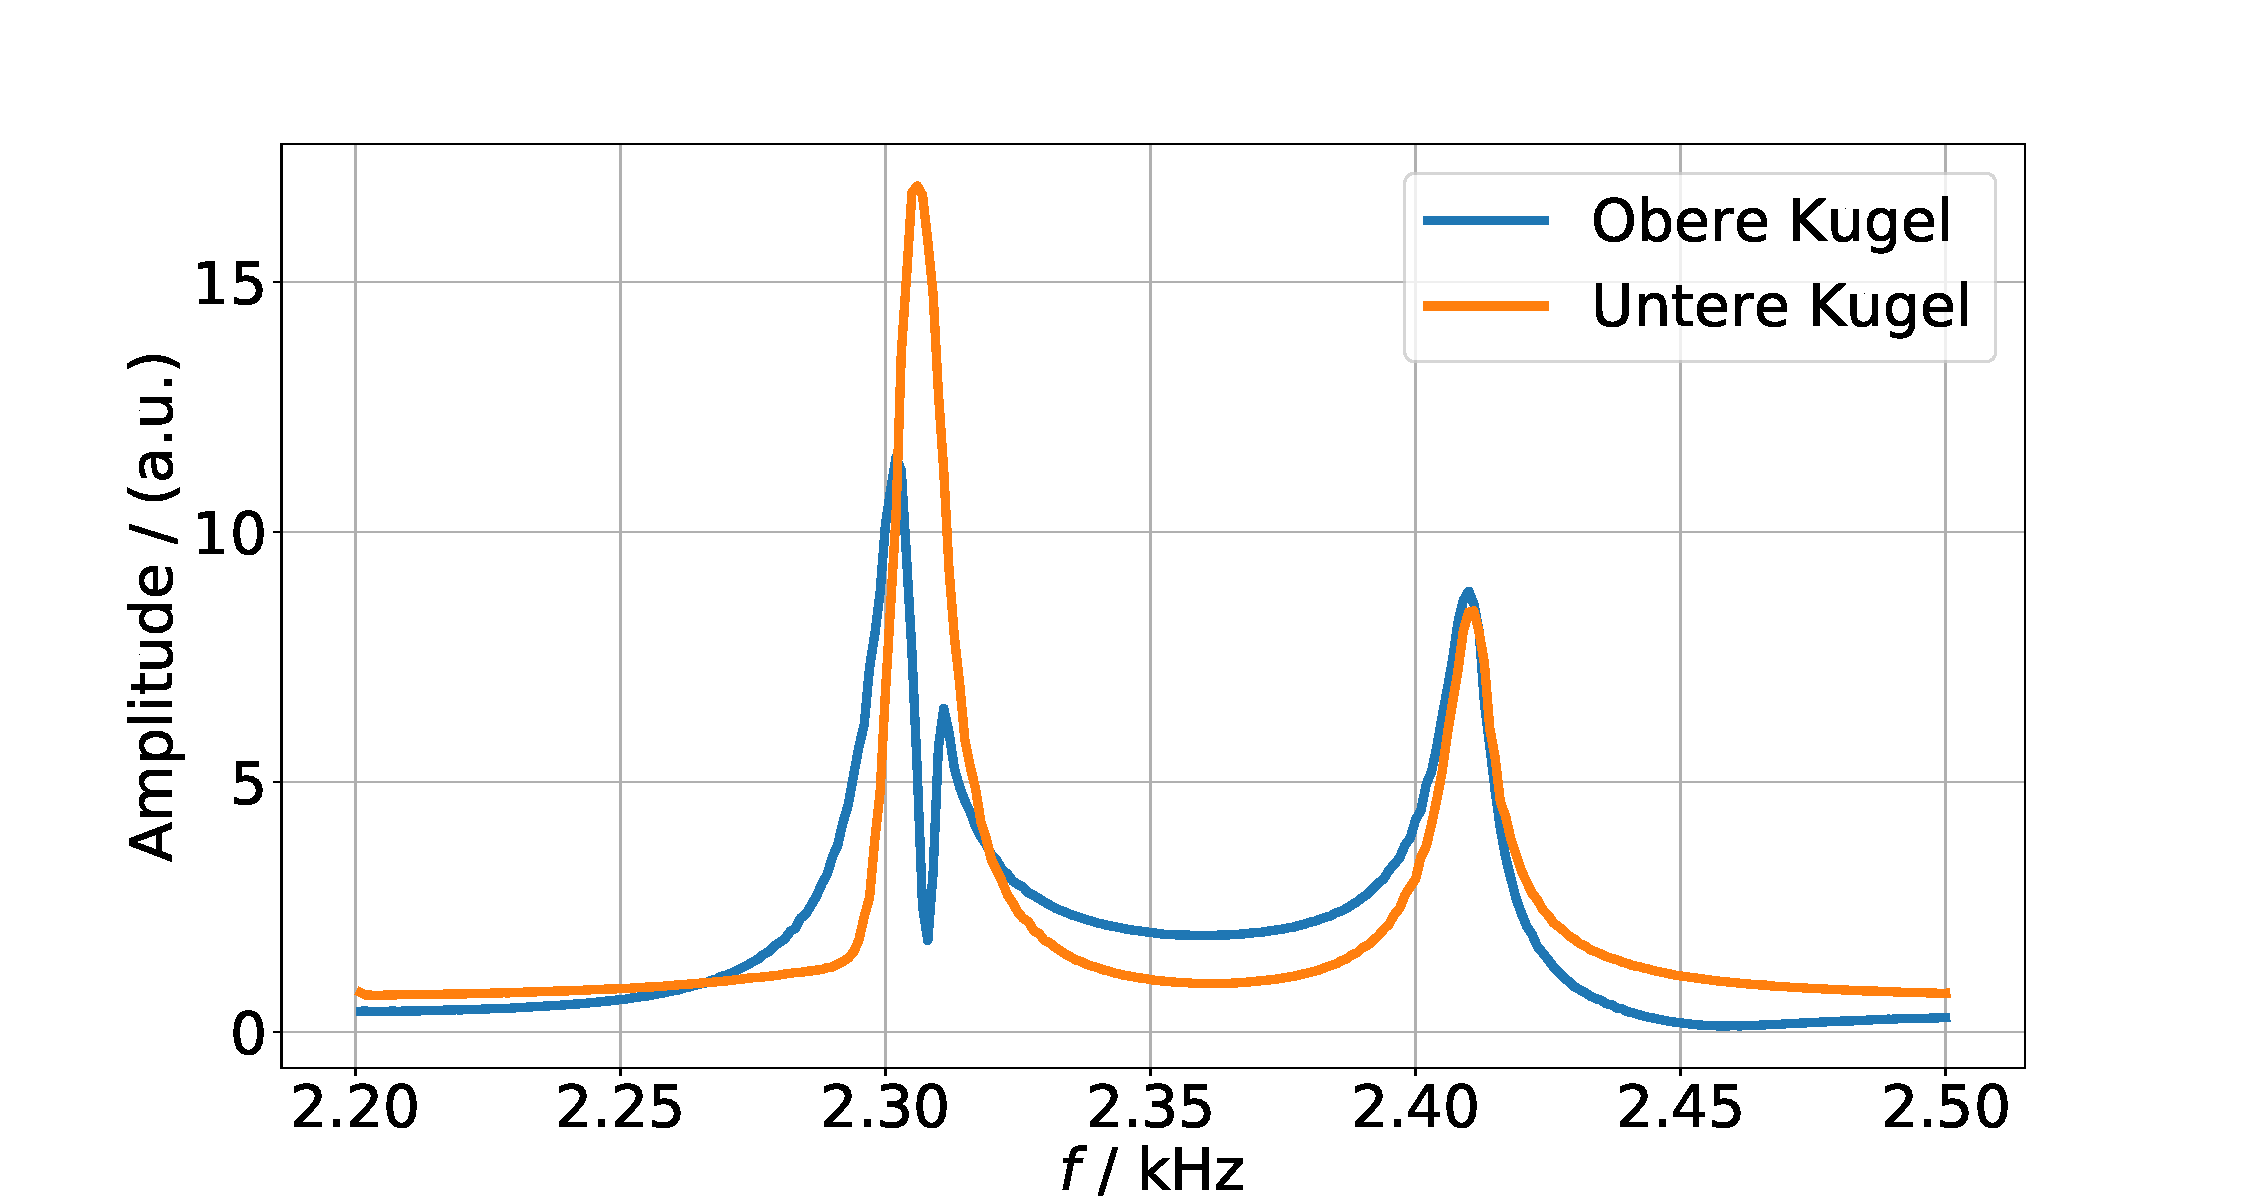
\includegraphics[width=0.7\textwidth]{plots/D_phase.pdf}
    \caption{Zu sehen ist das Frequenzspektrum um \SI{2.3}{\kilo\hertz} für den aus zwei Kugeln bestehenden Resonator. Hier ist die Messung der oberen und unteren Kugel zu sehen.}
    \label{fig:phase}
\end{figure}